\chapter{Inner Product Spaces}

In Chapter \ref{chap:vec_space}, we have discussed about what it means to be a vector space. Previously, it is accompanied by the dot product operation as defined in Section \ref{section:dotprod} that gives rise to the notion of \textit{Euclidean} distance in $\mathbb{R}^n$ (complex dot product for $\mathbb{C}^n$). In this chapter, we will show that the usual dot product is not the only way to measure distance between vectors: we can equip any vector space with a so-called \textit{inner product} that fulfills certain criteria and leads to an alternative expression for the length of vectors, in place of the dot product. This generalizes a vector space to an \textit{inner product space}, and many concepts for a vector space, like orthogonality, can be adapted to be applied in inner product spaces. Particularly, we will have the \textit{adjoint} as an inner product space equivalent to the usual transpose. Finally, we will talk about \textit{special polynomials} which are generated by considering suitable inner products and are often used in Earth Science applications, such as solving \textit{partial differential equations (PDEs)}.

\section{Definition and Properties of Inner Product Spaces}

\subsection{Requirements of Inner Products}

As introduced in the beginning, an \index{Inner Product Space}\keywordhl{inner product space} is a vector space (either real or complex) that comes with an \index{Inner Product}\keywordhl{inner product} operation that is akin to the usual dot product. To qualify as a valid inner product, it has to fulfill four requirements as suggested below.
\begin{defn}[Inner Product (Space)]
\label{defn:innerprod}
An inner product on a vector space $\mathcal{V}$ over $\mathbb{R}$ ($\mathbb{C}$) is a function that takes a pair of vectors $\vec{u}, \vec{v} \in \mathcal{V}$ as the input and returns an $\mathbb{R}$ ($\mathbb{C}$) number, denoted by $\langle \vec{u}, \vec{v} \rangle$. Then, for any $\vec{u}, \vec{v}, \vec{w} \in \mathcal{V}$ and scalar $a \in \mathbb{R}$ ($\mathbb{C}$), the following four axioms have to hold.
\begin{enumerate}
    \item $\langle \vec{u}, \vec{v} \rangle = \langle \vec{v}, \vec{u} \rangle$ ($\langle \vec{u}, \vec{v} \rangle = \overline{\langle \vec{v}, \vec{u} \rangle}$) ((Conjugate) Symmetry);
    \item $\langle \vec{u}+\vec{v}, \vec{w} \rangle = \langle \vec{u}, \vec{w} \rangle + \langle \vec{v}, \vec{w} \rangle$ (Additivity);
    \item $\langle a\vec{u}, \vec{v} \rangle = a\langle \vec{u}, \vec{v} \rangle$ (Homogeneity); and
    \item $\langle \vec{v}, \vec{v} \rangle \geq 0$, and $\langle \vec{v}, \vec{v} \rangle = 0$ if and only if $\vec{v} = \textbf{0}$ is the zero vector. (Positivity)
\end{enumerate}
The second and third condition can be combined into \textit{linearity}: given another scalar $b \in \mathbb{R}$ ($\mathbb{C}$), we have $\langle a\vec{u}+b\vec{v}, \vec{w} \rangle = a\langle \vec{u}, \vec{w} \rangle + b\langle \vec{v}, \vec{w} \rangle$. A real (complex) vector space with an inner product is then known as a real (complex) inner product space. 
\end{defn}
Short Exercise: Show that $\langle a\vec{u}, b\vec{v} \rangle = a\bar{b}\langle \vec{u}, \vec{v} \rangle$ for any complex inner product space.\footnote{$\langle a\vec{u}, b\vec{v} \rangle = a\langle \vec{u}, b\vec{v} \rangle = a\overline{\langle b\vec{v}, \vec{u} \rangle} = a\overline{b\langle \vec{v}, \vec{u} \rangle} = a\bar{b} \overline{\langle \vec{v}, \vec{u} \rangle} = a\bar{b}\langle \vec{u}, \vec{v} \rangle$ by the first and third axiom.}\par
For now, we will limit ourselves to finite-dimensional vector/inner product spaces until Section \ref{section:infinner}. It is not hard to verify that the above axioms hold for the usual dot product, so $\mathbb{R}^n$ (as well as $\mathbb{C}^n$) is automatically an inner product space when the (complex) dot product is equipped. In this case they are known as the \index{Standard Inner Product}\keywordhl{standard inner product} and \index{Euclidean $n$-space}\keywordhl{Euclidean $n$-space}. However, $\mathbb{R}^n$ will be a different inner product space when another inner product is used. It can be shown that all alternative inner products that can applied to $\mathbb{R}^n$ are precisely positive-definite symmetric bilinear forms as the extension of positive-definite quadratic forms introduced in the last chapter. Given such a positive-definite quadratic form $B$, then it can be verified that $\langle \vec{u}, \vec{v} \rangle = \vec{u}^TB\vec{v}$ will satisfy the real inner product axioms.\footnote{For (1): $\langle \vec{u}, \vec{v} \rangle = \vec{u}^TB\vec{v} = (\vec{u}^TB\vec{v})^T$ since it is only a scalar, and then $(\vec{u}^TB\vec{v})^T = \vec{v}^TB^T\vec{u} = \vec{v}^TB\vec{u} = \langle \vec{v}, \vec{u} \rangle$ as $B$ is symmetric. (2) and (3) are obvious. For (4), as $B$ is required to be positive-definite, $\langle \vec{v}, \vec{v} \rangle = \vec{v}^TB\vec{v} > 0$ by Definition \ref{defn:quaddefinite} as long as $\vec{v} \neq \textbf{0}$ and it is apparent that $\langle \vec{v}, \vec{v} \rangle = \textbf{0}B\textbf{0} = 0$ when $\vec{v} = \textbf{0}$.} Below are some other properties of inner product extended from the axioms that can be compared to Properties \ref{proper:dotproper} and \ref{proper:complexdot}.
\begin{proper}
\label{proper:innerprod2}
For vectors $\vec{u}, \vec{v}, \vec{w} \in \mathcal{V}$ and scalar $b \in \mathbb{R}$ ($\mathbb{C}$) in a real (complex) inner product space, we have
\begin{enumerate}
    \item $\langle \vec{u} \pm \vec{v}, \vec{w} \rangle = \langle \vec{u}, \vec{w} \rangle \pm \langle \vec{v}, \vec{w} \rangle$;
    \item $\langle \vec{u}, \vec{v} \pm \vec{w} \rangle = \langle \vec{u}, \vec{v} \rangle \pm \langle \vec{u}, \vec{w} \rangle$;
    \item $\langle \vec{v}, \textbf{0} \rangle = \langle \textbf{0}, \vec{v} \rangle = 0$;
    \item $\langle \vec{u}, b\vec{v} \rangle = b\langle \vec{u}, \vec{v} \rangle$ ($\langle \vec{u}, b\vec{v} \rangle = \bar{b}\langle \vec{u}, \vec{v} \rangle$);
    \item if $\langle \vec{u}, \vec{v} \rangle = \langle \vec{u}, \vec{w} \rangle$ for all $\vec{u}$, then $\vec{v} = \vec{w}$.
\end{enumerate}
\end{proper}
\begin{proof}
We will skip (1). (2): $\langle \vec{u}, \vec{v} \pm \vec{w} \rangle = \overline{\langle \vec{v} \pm \vec{w}, \vec{u} \rangle} = \overline{\langle \vec{v}, \vec{u} \rangle} \pm \overline{\langle \vec{w}, \vec{u} \rangle} = \langle \vec{u}, \vec{v} \rangle \pm \langle \vec{u}, \vec{w} \rangle$ by the first and second axiom. (3): $\langle \textbf{0}, \vec{v} \rangle = \langle 0\vec{u}, \vec{v} \rangle = 0\langle \vec{u}, \vec{v} \rangle = 0$ using arbitrary $\vec{u}$ and the third axiom. (4) simply follows from the last short exercise with $a = 1$. For (5):
\begin{align*}
\langle \vec{u}, \vec{v} \rangle &= \langle \vec{u}, \vec{w} \rangle \\
\langle \vec{u}, \vec{v} - \vec{w} \rangle &= 0 & \text{(By (1))}
\end{align*}
Then by letting $\vec{u} = \vec{v} - \vec{w}$ and using the last axiom we get $\vec{v} - \vec{w} = \textbf{0}$ and thus $\vec{v} = \vec{w}$.
\end{proof}

\subsection{Generalization of Length and Orthogonality via Inner Products}

As noted earlier, the idea of inner products extends the usual dot product and we may ask how the notion of vector length, which can be expressed via the dot product of the vector with itself (Properties \ref{proper:lengthdot}), is carried over to an inner product space. The most natural generalization is to simply replace the dot product by an inner product in Properties \ref{proper:lengthdot} when computing such a "length", which is now more properly known as a \index{Norm}\keywordhl{norm}. This makes physical sense as the last axiom in Definition \ref{defn:innerprod} forces the norm to always be positive ($0$ if it is the zero vector) just like the usual length.
\begin{proper}
\label{proper:norminner}
The norm of a vector in an inner product space is induced by
\begin{align*}
\norm{\vec{v}} &= \sqrt{\langle\vec{v} , \vec{v}\rangle} & &\text{or equivalently} &
\norm{\vec{v}}^2 &= \langle\vec{v} , \vec{v}\rangle
\end{align*}
\end{proper}
Unit vectors are then conveniently created using this definition of norm.
\begin{defn}
\label{defn:unitvecinner}
The unit vector of a non-zero vector $\vec{v}$ in an inner product space is denoted as $\hat{v}$ and is given by
\begin{align*}
\hat{v} &= \frac{1}{\norm{\vec{v}}}\vec{v}
\end{align*}
where the norm $\norm{\vec{v}}$ is now defined as in Properties \ref{proper:norminner}. 
\end{defn}
The notion of orthogonality in Properties \ref{proper:dotorth} is also transferred to an inner product space by the same essence of replacing the dot product by an inner product.
\begin{proper}
\label{proper:orthoinner}
Two vectors $\vec{u}, \vec{v} \in \mathcal{V}$ in an inner product space are said to be orthogonal with respect to the inner product when $\langle\vec{u} , \vec{v}\rangle = \langle\vec{v} , \vec{u}\rangle = 0$.
\end{proper}
Some other related results derived using dot product are also valid when inner products are used instead and we note them below.
\begin{thm}[Cauchy–Schwarz Inequality]
\label{thm:cauchyschinner}
Given two vectors $\vec{u}, \vec{v} \in \mathcal{V}$ in an inner product space, we have
\begin{align*}
\abs{\langle\vec{u} , \vec{v}\rangle} \leq \norm{\vec{u}}\norm{\vec{v}} =  \sqrt{\langle\vec{u} , \vec{u}\rangle} \sqrt{\langle\vec{v} , \vec{v}\rangle}
\end{align*}
\end{thm}
The proof is essentially the same as the one in Theorem \ref{thm:CauchySch} but with all the dot product expressions replaced by the inner product. Also
\begin{proper}
Non-zero orthogonal vectors with respect to any inner product are linearly independent.
\end{proper}
Again, the proof follows the same line of arguments as in Properties \ref{proper:ortholinind} with the dot product changed to an inner product.

\begin{exmp}
Show that $\vec{u} = (1,2)^T$ and $\vec{v} = (-3,4)^T$ in $\mathbb{R}^2$ are orthogonal to each other if the inner product used is given by
\begin{align*}
\langle\vec{u}, \vec{v}\rangle = \vec{u}^TB\vec{v}
\end{align*}
where 
\begin{align*}
B = 
\begin{bmatrix}
2 & 1 \\
1 & 1
\end{bmatrix}
\end{align*}
\end{exmp}
\begin{solution}
First we have to make sure the inner product defined as a symmetric bilinear form above is indeed valid, particularly it has to be positive-definite. By Theorem \ref{thm:quaddefinite}, it simply amounts to check if the eigenvalues are all positive. A simple calculation reveals that $\lambda = \frac{3+\sqrt{5}}{2}, \frac{3-\sqrt{5}}{2} > 0$ so we can proceed to calculate
\begin{align*}
\langle\vec{u}, \vec{v}\rangle &= \vec{u}^TB\vec{v} \\
&= \begin{bmatrix}
1 & 2
\end{bmatrix}
\begin{bmatrix}
2 & 1 \\
1 & 1
\end{bmatrix}
\begin{bmatrix}
-3 \\
4
\end{bmatrix} \\
&= \begin{bmatrix}
1 & 2
\end{bmatrix}
\begin{bmatrix}
-2 \\
1
\end{bmatrix} = 0
\end{align*}
Hence by Properties \ref{proper:orthoinner} the two vectors are orthogonal with respect to the said inner product. Obviously they will not be orthogonal if the usual dot product is used instead.
\end{solution}

\subsection{Infinite-dimensional Inner Product Spaces}
\label{section:infinner}

We have been staying in the realm of finite-dimensional vector/inner product spaces until now but the utility of inner product spaces only become the most significant when they are infinite-dimensional. As suggested by Properties \ref{proper:samenvecsbases}, if there is a basis for an infinite-dimensional vector space\footnote{Actually, there always exists some basis for any infinite-dimensional vector space due to the \textit{Zorn's Lemma}, or equivalently the \textit{Hausdorff's Maximal Principle}.}, it must be infinite. An example of infinite-dimensional inner product spaces will be $\mathcal{C}^0[a,b]$, the vector space of all continuous functions in one variable over the interval $a \leq x \leq b$, equipped with the frequently used inner product of
\begin{align}
\langle f,g \rangle = \int_a^b f(x) \overline{g(x)} dx \label{eqn:integralinner}
\end{align}
where $a < b$ are some real constants. Checking the validity of this inner product formulation is not hard.\footnote{We will only justify (4) in Definition \ref{defn:innerprod} and leave the remaining axioms to the readers. It is obvious that if $f(x) = 0$ is the zero function then $\langle f,f \rangle = \int_a^b (0)^2 dx = 0$. Assume that $f(x)$ is not everywhere zero, then by continuity from elementary calculus, we know that $f(c) \neq 0$ and hence $\abs{f(c)}^2 > 0$ at some point $a \leq c \leq b$ and there exists $\delta > 0$ such that $\abs{f(x)}^2 > \frac{\abs{f(c)}^2}{2}$ where $c-\delta \leq c \leq c+\delta$, therefore $\langle f,f \rangle \geq \frac{\abs{f(c)}^2}{2} (2\delta) = \abs{f(c)}^2 \delta > 0$.} 
Unfortunately, the above example lacks the most desirable attribute of being a \index{Hilbert Space}\keywordhl{Hilbert space}. The detailed explanation of how Hilbert spaces work belongs to the area of Functional Analysis and is very much out of the scope of this book\footnote{To put shortly, a Hilbert space is a \textit{complete} inner product space where all \textit{Cauchy sequences} are convergent. The meaning of complete here is different from that in Properties \ref{proper:hilbertorthosys}.}, and we will take the liberty to assume that an infinite-dimensional inner product space we work on is a \textit{separable} Hilbert space from time to time. For instance, the $L^2[a,b]$ space for all square-integrable functions\footnote{A square-integrable function $f$ means that $\int \abs{f}^2 < \infty$ is finite, and the $L^2[a,b]$ space is actually the "completed" (in the sense of the footnote above) version of $\mathcal{C}^0[a,b]$.} equipped with the same inner product in Equation (\ref{eqn:integralinner}) is such a Hilbert space. The reason why we care so much about Hilbert spaces, particularly those are separable, is that they always admit a countable orthonormal basis that is complete.
\begin{proper}
\label{proper:hilbertorthosys}
An infinite-dimensioal separable Hilbert space $\mathcal{H}$ always have a countably infinite orthonormal basis $\{\varphi_j\}_{j=1}^{\infty}$ where $\varphi_j$ denotes the $j$-th basis vector and $j$ is an integer enumerated from $1$ to infinity. It is \textit{complete} in the sense that there exists no more other non-zero vector $\tilde{\varphi}$ can be included in the basis such that $\langle \tilde{\varphi}, \varphi_j \rangle = 0$ for all $j$ without making the set linearly dependent.
\end{proper}
Equivalently, it means that any vector/function in the Hilbert space can be expanded into an infinite sum\footnote{For an infinite-dimensional vector space, we often loosen the restriction so that an infinite sum of basis vectors is also regarded to constitute the span (see \textit{Schuader basis}).} of orthonormal vectors $f = c_1\varphi_1 + c_2\varphi_2 + \cdots = \sum_{j=1}^{\infty} c_j \varphi_j$.\footnote{(Note: again this only holds if the Hilbert space is \textit{separable}, but we will not go into the details.) If there exists such a vector $\tilde{\varphi}$ that satisfies $\langle \tilde{\varphi}, \varphi_j \rangle = 0$ for all $j$, then consider $f = \tilde{\varphi}$ and take the inner product with $\tilde{\varphi}$ on both sides. All the terms on R.H.S. will become zero but the L.H.S. is $\langle \tilde{\varphi}, \tilde{\varphi} \rangle > 0$ by the last axiom in Definition \ref{defn:innerprod}, a contradiction.} As noted before, the formal treatment of Hilbert spaces is out of our reach and we will invoke the relevant properties as we see fit.\par
Back to infinite-dimensional inner product spaces in general, the properties and theorems given earlier this section still hold for them as we have defined inner products in a way without regard to the (in)finiteness of dimensions.
\begin{exmp}
Verify that the Cauchy-Schwarz Inequality (Theorem \ref{thm:cauchyschinner}) holds for $\varphi_1 = x$ and $\varphi_2 = x^2$ in the $\mathcal{C}^0[0,1]$ space where the inner product is defined by Equation (\ref{eqn:integralinner}).
\end{exmp}
\begin{solution}
This is to check 
\begin{align*}
\abs{\langle\varphi_1 , \varphi_2\rangle} &\leq \norm{\varphi_1}\norm{\varphi_2} \\
\abs{\langle x , x^2\rangle} &\leq \norm{x}\norm{x^2}
\end{align*}
by computing the three quantities in the above inequality:
\begin{align*}
\abs{\langle x , x^2\rangle} &= \abs{\int_0^1 x \overline{(x^2)} dx} \\
&= \abs{\int_0^1 x^3 dx} \\
&= \abs{[\frac{1}{4}x^4]_0^1} = \abs{\frac{1}{4}} = \frac{1}{4} \\
\norm{x} &= \sqrt{\int_0^1 x \overline{(x)} dx} \\
&= \sqrt{\int_0^1 x^2 dx} \\
&= \sqrt{[\frac{1}{3}x^3]_0^1} = \sqrt{\frac{1}{3}} =\frac{1}{\sqrt{3}}
\end{align*}
similarly $\norm{x^2} = \frac{1}{\sqrt{5}}$. Hence $\abs{\langle x , x^2\rangle} = \frac{1}{4} = \frac{1}{\sqrt{16}} < \frac{1}{\sqrt{15}} = (\frac{1}{\sqrt{3}})(\frac{1}{\sqrt{5}}) = \norm{x}\norm{x^2}$ and the inequality holds in this case.
\end{solution}
Short Exercise: Show that the same\footnote{Actually they are not the same functions as before since their domain changes from $[0,1]$ to $[-1,1]$, but we use the word for the sake of convenience.} two functions $\varphi_1 = x$ and $\varphi_2 = x^2$ become orthogonal to each other in $\mathcal{C}^0[-1,1]$ where the inner product still takes the same form of Equation (\ref{eqn:integralinner}) but integrated from $-1$ to $1$ instead.\footnote{$\int_{-1}^1 x \overline{(x^2)} = \int_{-1}^1 x^3 = 0$ as $x^3$ is an odd function and the integration limits are symmetric.}

\section{Adjoints and Hermitian/Unitary Operators}

\subsection{Definition of Adjoints}

With the usual (complex) dot product as the inner product for $\mathbb{R}^n$ ($\mathbb{C}^n$), we have $\langle A\vec{u}, \vec{v} \rangle = \langle \vec{u}, A^T\vec{v} \rangle$ ($\langle \vec{u}, A^*\vec{v} \rangle$) by Properties \ref{proper:dotproper} (\ref{proper:complexdotherm}). Here the square matrix $A$ in the first argument can be moved to the second argument by applying a (conjugate) transpose on it. In this context, $A^T$ ($A^*$) is known as the \keywordhl{adjoint} of $A$ with respect to the dot product. Since any square matrix essentially represents a linear operator behind the scene (see Chapter \ref{chap:6x}), we can extend this idea for a vector space $\mathcal{V}$ in general, where $\vec{u}, \vec{v} \in \mathcal{V}$ and the linear operator is $T: \mathcal{V} \to \mathcal{V}$ now. Subsequently, the adjoint of $T$ will then be another linear operator $T^*$ defined by the relationship $\langle T(\vec{u}), \vec{v} \rangle = \langle \vec{u}, T^*(\vec{v}) \rangle$. Again, if the standard inner product is employed, then we know that if the matrix representation of $T$ in the basis $\beta$ is $[T]_\beta$, then
\begin{align*}
\langle T(\vec{u}), \vec{v} \rangle &\equiv \langle [T]_\beta[\vec{u}]_\beta, [\vec{v}]_\beta \rangle \\ 
&= \langle [\vec{u}]_\beta, ([T]_\beta)^*[\vec{v}]_\beta \rangle \stackrel{\text{def}}{\equiv} \langle \vec{u}, T^*(\vec{v}) \rangle
\end{align*}
so that we identify the adjoint operator $T^*$ with a conjugate transpose matrix representation of $([T]_\beta)^*$. 
\begin{defn}[Adjoint]
\label{defn:adjoint}
The adjoint of a linear operator $T: \mathcal{V} \to \mathcal{V}$ with respect to some inner product $\langle \;, \;\rangle$ is another linear operator denoted by $T^*$ such that
\begin{align*}
\langle T(\vec{u}), \vec{v} \rangle = \langle \vec{u}, T^*(\vec{v}) \rangle    
\end{align*}
holds for all $\vec{u}, \vec{v} \in \mathcal{V}$. Such an adjoint $T^*$ is always unique for a given $T$. 
\end{defn}
It is easy to check the linearity and uniqueness of an adjoint.\footnote{Linearity (Definition \ref{defn:lintrans}): Consider $\langle \vec{u}, T^*(a\vec{v} + b\vec{w}) \rangle = \langle T(\vec{u}), a\vec{v} + b\vec{w} \rangle = a\langle T(\vec{u}), \vec{v} \rangle + b\langle T(\vec{u}), \vec{w} \rangle$ by Definitions \ref{defn:adjoint} and \ref{defn:innerprod}. Subsequently $a\langle T(\vec{u}), \vec{v} \rangle + b\langle T(\vec{u}), \vec{w} \rangle = a\langle \vec{u}, T^*(\vec{v}) \rangle + b\langle \vec{u}, T^*(\vec{w}) \rangle = \langle \vec{u}, aT^*(\vec{v}) \rangle + \langle \vec{u}, bT^*(\vec{w}) \rangle = \langle \vec{u}, aT^*(\vec{v}) + bT^*(\vec{w}) \rangle$ by those definitions again. Since this has to hold for any $\vec{u}$ (plus $\vec{v}$ and $\vec{w}$), $\langle \vec{u}, T^*(a\vec{v} + b\vec{w}) \rangle = \langle \vec{u}, aT^*(\vec{v}) + bT^*(\vec{w}) \rangle$ means that $T^*(a\vec{v} + b\vec{w}) = aT^*(\vec{v}) + bT^*(\vec{w})$ by Properties \ref{proper:innerprod2}. Uniqueness: Assume that there is another adjoint $S^*$ satisfies $\langle T(\vec{u}), \vec{v} \rangle = \langle \vec{u}, S^*(\vec{v}) \rangle$ for all $\vec{u}$ and $\vec{v}$, then by Properties \ref{proper:innerprod2} $T^*(\vec{v}) = S^*(\vec{v})$ for all $\vec{v}$. Hence $T^*$ and $S^*$ must be the same operator.} Now let's look at how adjoint is found when inner products other than the standard one are used. First, if $\mathcal{V}$ is a finite-dimensional complex vector space and a new inner product is defined via a positive-definite Hermitian form $\langle \vec{u}, \vec{v} \rangle = \vec{u}^TB\overline{\vec{v}} = (B^T\vec{u})\cdot\overline{\vec{v}}$, then for a linear operator $T$ with a matrix representation of $[T]_\beta$ in the $\beta$ system, by Definition \ref{defn:complexdotproduct} and Properties \ref{proper:complexdotherm}:
\begin{align*}
\langle T(\vec{u}), \vec{v} \rangle &\equiv (B^T[T]_\beta[\vec{u}]_\beta) \cdot ([\vec{v}]_\beta) \\
&= (B^T[T]_\beta (B^T)^{-1} B^T [\vec{u}]_\beta) \cdot ([\vec{v}]_\beta) \\
&= (B^T[\vec{u}]_\beta) \cdot ((B^T[T]_\beta (B^T)^{-1})^*[\vec{v}]_\beta) \\
&\equiv \langle \vec{u}, (B^T[T]_\beta (B^T)^{-1})^* \vec{v} \rangle = \langle \vec{u}, (\overline{B})^{-1} [T]_\beta^* \overline{B} \vec{v} \rangle
\end{align*}
and thus we identify the matrix representation of the adjoint as $T^* \equiv (\overline{B})^{-1} [T]_\beta^* \overline{B}$ (notice that $[T]_\beta^*$ and $[T^*]_\beta$ are not the same) with respect to such an inner product. For an infinite-dimensional inner product space, the inner product used is usually in the form of an integral like the one in Equation (\ref{eqn:integralinner}), additionally with a weighting function, and a linear operator $T$ can be more general, including differentiation and multiplication by some function, or a mix of them. As a result, the adjoint is often found via the technique of \textit{integration by parts}, producing boundary terms as a by-product. Conventionally, we will use $\mathcal{L}$ in place of $T$ to denote the operator when the vectors are functions.
\begin{proper}
\label{proper:adjointinnerint}
For a general integral inner product:
\begin{align}
\langle f,g \rangle = \int_a^b w(x) f(x) \overline{g(x)} dx \label{eqn:integralinner2}
\end{align}
where $w(x) > 0$ is a positive-definite \textit{real} weighting function, the unique adjoint $\mathcal{L}^*$ of a linear operator $\mathcal{L}$ is another one that satisfies
\begin{align*}
\langle f,\mathcal{L}[g] \rangle &= \int_a^b w(x) f(x) \overline{(\mathcal{L}[g(x)])} dx \\ 
&= \int_a^b w(x) \mathcal{L}^*[f(x)] \overline{g(x)} dx + \text{boundary terms} \\
&= \langle \mathcal{L}^*[f],g \rangle + \text{boundary terms}
\end{align*}
for all functions $f, g \in \mathcal{V}$ and the boundary terms are evaluated at the end-points $a$ and $b$.
\end{proper}
Equation (\ref{eqn:integralinner}) is then simply a special case of (\ref{eqn:integralinner2}) with a constant weight of $w = 1$.
\begin{exmp}
Find the adjoint of the linear operator $\mathcal{L}[f] = x\frac{d}{dx}[f]$ with respect to the inner product in Equation (\ref{eqn:integralinner}).
\end{exmp}
\begin{solution}
We start with $\langle f,\mathcal{L}[g] \rangle = \int_a^b f(x) \overline{\left(x\frac{d}{dx}(g(x))\right)} dx$ and aim to rewrite it into the form of $\int_a^b \mathcal{L}^*[f(x)] \overline{g(x)} dx = \langle \mathcal{L}^*[f],g \rangle$, plus possibly some boundary term(s). As suggested by above we can try to apply integration by parts:
\begin{align*}
\langle f,\mathcal{L}[g] \rangle &= \int_a^b f(x) \overline{\left(x\frac{d}{dx}(g(x))\right)} dx \\  
&= \int_a^b xf(x) \frac{d}{dx}\overline{(g(x))} dx \\
&= [xf(x)\overline{(g(x))}]_a^b - \int_a^b \frac{d}{dx}(xf(x))\overline{(g(x))} dx \\
&= \int_a^b -\frac{d}{dx}(xf(x))\overline{(g(x))} dx + [xf(x)\overline{(g(x))}]_a^b
\end{align*}
After rearrangement, the boundary term is put after the integral, from which we deduce that $\mathcal{L}^*[f] = -\frac{d}{dx}(x[f])$ by comparing it with $\int_a^b \mathcal{L}^*[f(x)] \overline{g(x)} dx$.
\end{solution}
Finally we note some properties of adjoints that can be compared to Properties \ref{proper:complexmat}.
\begin{proper}
For two linear operators $T$ and $U$ in the same inner product space with adjoints $T^*$ and $U^*$ respectively, we have
\begin{enumerate}
\item $(cT)^* = \overline{c}T^*$, where $c$ is any complex scalar,
\item $(T^*)^* = T$,
\item $(T \pm U)^* = T^* \pm U^*$,
\item $(TU)^* = U^*T^*$.
\end{enumerate}
\end{proper}
We will briefly show the last item here. Using Definition \ref{defn:adjoint} twice, we have
\begin{align*}
\langle TU(\vec{u}), \vec{v} \rangle &= \langle U(\vec{u}), T^*(\vec{v}) \rangle \\
&= \langle \vec{u}, U^*T^*(\vec{v}) \rangle
\end{align*}
so we identify that $(TU)^* = U^*T^*$.

\subsection{Hermitian Operators}
As suggested by the last subsection, adjoints are the inner product counterpart of (conjugate) transposes. Therefore, it is natural to ask if the concept of symmetric or Hermitian in the matrix world is also applicable to an adjoint. Correspondingly, when a linear operator $T$ has an adjoint $T^*$ which is equal to itself, i.e.\ $T^* = T$, it is called \index{Self-adjoint}\keywordhl{self-adjoint}, as the inner product equivalent of Hermitian. If the inner product space is finite-dimensional with a positive-definite Hermitian form $B$ as its inner product, then according to what we have just derived we simply need to check if $T^* \equiv (\overline{B})^{-1} [T]_\beta^* \overline{B} = [T]_\beta \equiv T$. The problem becomes a bit more complicated when we consider the integral inner product in Equation (\ref{eqn:integralinner2}) because even when $\mathcal{L}^* = \mathcal{L}$ is self-adjoint there can be boundary terms. We need an even stronger condition where there is no boundary term so that $\mathcal{L}$ becomes "nicer" to work with and gives desirable properties. In this situation, the self-adjoint $\mathcal{L}$ is further known as a \index{Hermitian}\keywordhl{Hermitian} operator.
\begin{defn}
\label{defn:selfadjoint}
A linear operator $T$ is self-adjoint if its adjoint $T^* = T$ equals to itself. A linear operator $\mathcal{L}$ is Hermitian if it is self-adjoint and all boundary terms vanish.
\end{defn}
The absence of any boundary term can be due to the structure of $\mathcal{L}$ or $\mathcal{L}^*$ itself, or the boundary condition(s) imposed on the input functions. 
\begin{exmp}
Show that $\mathcal{L} = -i \hbar\frac{d}{dx}$, where $\hbar$ is a real constant, is a self-adjoint operator with respect to the inner product in Equation (\ref{eqn:integralinner}) over the entire $x$-axis. Find the form of its eigenfunctions (treating functions as (eigen)vectors).
\end{exmp}
\begin{solution}
\begin{align*}
\langle f,\mathcal{L}[g] \rangle &= \int_{-\infty}^\infty f(x) \overline{(\mathcal{L}[g(x)])} dx \\
&= \int_{-\infty}^\infty f(x) \overline{\left(-i \hbar\frac{d}{dx}(g(x))\right)} dx \\
&= \int_{-\infty}^\infty i\hbar f(x) \frac{d}{dx}(g(x)) dx \\
&= [i\hbar f(x)g(x)]_{-\infty}^\infty - \int_{-\infty}^\infty i\hbar \frac{d}{dx}(f(x)) g(x) dx & \text{(Integration by parts)} \\
&= \int_{-\infty}^\infty -i\hbar \frac{d}{dx}(f(x)) g(x) dx + [i\hbar f(x)g(x)]_{-\infty}^\infty \\
&= \int_{-\infty}^\infty \mathcal{L}[f(x)] g(x) dx + [i\hbar f(x)g(x)]_{-\infty}^\infty
\end{align*}
So we see that $\mathcal{L}^* = \mathcal{L}$ is self-adjoint. The eigenfunctions $\varphi$ of $\mathcal{L}$ can be found from solving the ODE:
\begin{align*}
\mathcal{L}[\varphi] = -i \hbar\frac{d\varphi}{dx} &= m\varphi \\
-\int i \hbar \frac{d\varphi}{\varphi} &= \int m dx \\
- i \hbar \ln{\varphi} &= mx + C \\
\therefore \varphi &= Ke^{\frac{i}{\hbar}mx}
\end{align*}
where $K = e^{\frac{i}{\hbar} C}$ is any scaling constant. Notice that the eigenvalue $m$ can take any value ranging from $-\infty$ to $\infty$ as there is no boundary condition being enforced. In this case, the eigenvalues form a \textit{continuous spectrum} and we note that the vector space generated by those eigenfunctions, which are uncountable in this problem, are not separable. In fact, this operator $\mathcal{L} = -i \hbar\frac{d}{dx}$, is famously referred to as the \textit{momentum operator} in Quantum Mechanics.
\end{solution}
The above example shows that eigenfunctions for a self-adjoint linear operator may be uncountable. In this case, a function cannot be represented by an infinite sum $f = c_1\varphi_1 + c_2\varphi_2 + \cdots = \sum_{j=1}^{\infty} c_j \varphi_j$ as suggested by Properties \ref{proper:hilbertorthosys} but rather requires to be expressed by an integral $f(x) = \int_0^\infty c_m\varphi_m(x) dm$ over a continuous index $m$, which is much more troublesome to deal with. This is the exact reason why we introduce Hermitian operators in this part, as they carry the desirable properties of possessing countably infinite eigenfunctions that form a complete orthonormal basis and a \textit{discrete spectrum}, provided that the Hilbert space where the Hermitian operator acts on is already separable. The completeness of the eigenfunctions of a Hermitian operator, again should be delegated to the world of Functional Analysis.
But first, we can show an essential property of Hermitian operators that their eigenvalues are always real, which can be compared to Properties \ref{proper:hermrealeig}.
\begin{proper}
\label{proper:hermrealeiginner}
The eigenvalues of any Hermitian operator $T^* = T$ must be real.
\end{proper}
\begin{proof}
(WIP)
\end{proof}
Moreover, we can briefly prove the orthogonality between its eigenfunctions.
\begin{proper}
\label{proper:orthogonalherm}
Any two eigenfunctions of a Hermitian operator $\mathcal{L}^* = \mathcal{L}$ corresponding to two distinct eigenvalues are always orthogonal to each other.
\end{proper}
This closely parallels Properties \ref{proper:symortho} and the proof is also very similar.
\begin{proof}
Denote the two eigenfunctions as $\varphi_1$ and $\varphi_2$ where the respective eigenvalues are $m_1$ and $m_2$. Subsequently we have
\begin{align*}
\langle \varphi_1, \mathcal{L}[\varphi_2] \rangle &= \langle \varphi_1, m_2\varphi_2 \rangle \\
&= \bar{m_2} \langle \varphi_1, \varphi_2 \rangle = m_2 \langle \varphi_1, \varphi_2 \rangle & \text{(Properties \ref{proper:hermrealeiginner})}
\end{align*}
but also
\begin{align*}
\langle \varphi_1, \mathcal{L}[\varphi_2] \rangle &= \langle \mathcal{L}^*[\varphi_1], \varphi_2 \rangle & \text{(Properties \ref{proper:adjointinnerint})} \\
&= \langle \mathcal{L}[\varphi_1], \varphi_2 \rangle & \text{(Definition \ref{defn:selfadjoint})} \\
&= \langle m_1\varphi_1, \varphi_2 \rangle \\
&= m_1 \langle \varphi_1, \varphi_2 \rangle
\end{align*}
So
\begin{align*}
m_1 \langle \varphi_1, \varphi_2 \rangle &= m_2 \langle \varphi_1, \varphi_2 \rangle \\
(m_1 - m_2) \langle \varphi_1, \varphi_2 \rangle &= 0
\end{align*}
but the two eigenvalues are taken to be distinct, $m_1 \neq m_2$, hence it must be that $\langle \varphi_1, \varphi_2 \rangle$ = 0 and $\varphi_1, \varphi_2$ are orthogonal with respect to the inner product (Properties \ref{proper:orthoinner}).
\end{proof}
We can then divide the eigenfunctions by their norm as in Definition \ref{defn:unitvecinner} to make them have unit length and hence become orthonormal. Even when some of the $k$ eigenfunctions have the same eigenvalue (in this context they are said to be \textit{$k$-fold degenerate}), we can apply the Gram-Schmidt Orthogonalization process adapted for inner product space (to be discussed soon in Section \ref{section:GSorthinnersec}), over those eigenfunctions, in a fashion very similar to the idea suggested in the discussion below Properties \ref{proper:symortho}. Now let's see a very standard example of a Hermitian operator leading to a complete set of orthonormal eigenfunctions.
\begin{exmp}
\label{exmp:Fourierbasis}
For the separable Hilbert space $L^2[-\pi, \pi]$ of square-integrable functions along $-\pi \leq x \leq \pi$, show that the linear operator $\mathcal{L}[f] = \frac{d^2}{dx^2}[f]$ will be Hermitian with respect to the inner product in Equation (\ref{eqn:integralinner}) if the (eigen)functions are picked in a way so that the boundary terms vanish.
\end{exmp}
\begin{solution}
First, we have to check if $\mathcal{L}$ is self-adjoint, from
\begin{align*}
\langle f,\mathcal{L}[g] \rangle &= \int_{-\pi}^\pi f(x) \overline{(\mathcal{L}[g(x)])} dx \\  
&= \int_{-\pi}^\pi f(x) \overline{\frac{d^2}{dx^2}([g(x)])} dx \\
&= \int_{-\pi}^\pi f(x) \frac{d^2}{dx^2}\overline{([g(x)])} dx \\
&= [f(x) \frac{d}{dx}\overline{([g(x)])}]_{-\pi}^\pi - \int_{-\pi}^\pi \frac{d}{dx}(f(x)) \frac{d}{dx}\overline{([g(x)])} dx \\
&= [f(x) \frac{d}{dx}\overline{([g(x)])}]_{-\pi}^\pi - [\frac{d}{dx}(f(x)) \overline{g(x)}]_{-\pi}^\pi \\
&\quad + \int_{-\pi}^\pi \frac{d^2}{dx^2}(f(x)) \overline{g(x)} dx \\
&= [f(x) \frac{d}{dx}\overline{([g(x)])}]_{-\pi}^\pi - [\frac{d}{dx}(f(x)) \overline{g(x)}]_{-\pi}^\pi \\
&\quad + \int_{-\pi}^\pi \mathcal{L}(f(x)) \overline{g(x)} dx
\end{align*}
and thus $\mathcal{L}^* = \frac{d^2}{dx^2} = \mathcal{L}$. Again from basic ODE we know that the eigenfunctions $\varphi$ of $\mathcal{L}[f] = \frac{d^2}{dx^2}[f]$ will be in the form of $\sin(mx)$ and $\cos(mx)$ as $\frac{d^2}{dx^2}(\sin(mx)) = -m^2\sin(mx)$ and $\frac{d^2}{dx^2}(\cos(mx)) = -m^2\cos(mx)$. For the two boundary terms to vanish, $m = 0, 1, 2, \ldots$ must be a non-negative integer\footnote{Without loss of generality, let $f = \sin(m_1 x)$ and $g = \cos(m_2 x)$, then
\begin{align*}
&\quad [f(x) \frac{d}{dx}\overline{([g(x)])}]_{-\pi}^\pi - [\frac{d}{dx}(f(x)) \overline{g(x)}]_{-\pi}^\pi \\
&= [-m_2\sin(m_1 x)\sin(m_2 x)]_{-\pi}^\pi - [m_1\cos(m_1 x)\cos(m_2 x)]_{-\pi}^\pi \\
&= [-\frac{m_2}{2}(\cos((m_1-m_2)x) - \cos((m_1+m_2)x))]_{-\pi}^\pi \\
&\quad - [\frac{m_1}{2}(\cos((m_1-m_2)x) + \cos((m_1+m_2)x))]_{-\pi}^\pi 
\end{align*}
using trigonometric identities. From this we see that if the two boundary terms have to be zero, $m_1 - m_2$ and $m_1 + m_2$ must both be odd or even at the same time, which implies that $m_1$ and $m_2$ have to be integers. And since $\sin(-m_1 x) = -\sin(m_1 x)$ and $\cos(-m_2 x) = \cos(m_2 x)$, we only need to take the integers that are positive.}, and hence the countably infinite, orthogonal\footnote{Again, without the loss of generality, we let $f = \sin(m_1 x)$ and $g = \cos(m_2 x)$ where $m_1$ and $m_2$ are now positive integers. Then the orthogonality is verified by computing
\begin{align*}
\int_{-\pi}^{\pi} \sin(m_1 x)\cos(m_2 x) dx &= \int_{-\pi}^{\pi} \frac{1}{2} (\sin((m_1 - m_2)x) + \sin((m_1 + m_2)x)) dx \\
&= [\frac{1}{2} (-\frac{\cos((m_1 - m_2)x)}{m_1 - m_2} - \frac{\cos((m_1 + m_2)x)}{m_1 + m_2})]_{-\pi}^{\pi} 
\end{align*}
which yields $0$ when the end-points $-\pi, \pi$ are substituted into the expression.} (not yet normalized) basis of eigenfunctions are $\{\sin(x), \sin(2x), \sin(3x), \ldots, 1, \cos(x), \cos(2x), \cos(3x), \ldots\}$. This basis, consisting of sines and cosines with discrete, equally spaced frequencies, is famously known as the \index{Fourier Basis}\keywordhl{Fourier basis}.
\end{solution}

\subsection{Unitary Operators}

Another class of matrices we want to generalize for inner product spaces is the orthogonal/unitary one introduced in Chapter \ref{chap:normalmat}. For those matrices, let's say $A$, two defining properties are that $A^{-1} = A^*$ and the preservation of distance noted in Properties \ref{proper:ortholengthpreserve}. Therefore, we want a unitary operator $T$ to satisfy the same properties where $T^*$ is now its adjoint and the notion of distance is with respect to the given inner product.
\begin{defn}
\label{defn:unitaryop}
A unitary operator $T$ is a linear operator such that its inverse operator equals to its adjoint $T^{-1} = T^*$ with respect to the inner product used.
\end{defn}
With this definition, the distance-preserving property can be readily derived.
\begin{proper}
Transformation by a unitary operator $T$ on a vector is length-preserving.
\end{proper}
which should be compared to Properties \ref{proper:ortholengthpreserve}.
\begin{proof}
Denote the original vector as $\vec{v}$ and the newly transformed vector be $T(\vec{v})$, then its length, given as the norm in Properties \ref{proper:norminner},
\begin{align*}
\norm{T(\vec{v})}^2 = \langle T(\vec{v}), T(\vec{v}) \rangle &= \langle \vec{v}, T^*(T(\vec{v})) \rangle & \text{(Definition \ref{defn:adjoint})} \\
&= \langle \vec{v}, T^{-1}(T(\vec{v})) \rangle & \text{(Definition \ref{defn:unitaryop})} \\
&= \langle \vec{v}, \text{id}(\vec{v}) \rangle & \text{(Definition \ref{defn:inversetrans})} \\
&= \langle \vec{v}, \vec{v} \rangle = \norm{\vec{v}}^2
\end{align*}
is shown to be equal throughout the unitary transformation.
\end{proof}
\begin{exmp}
Show that for the $L^2[a,b]$ space with the inner product of Equation (\ref{eqn:integralinner}), the linear operator $\mathcal{L}[f] = e^{ikx}[f]$ where $k$ is any real number, is unitary.
\end{exmp}
\begin{solution}
It is apparent that the inverse of $\mathcal{L}$ is $\mathcal{L}^{-1}[f] = e^{-ikx}[f]$ so that $(\mathcal{L}^{-1} \circ \mathcal{L})[f] = e^{-ikx}(e^{ikx}[f]) = (1)f = \text{id}[f]$, and we have to show that it equals to the adjoint $\mathcal{L}^*$:
\begin{align*}
\langle f,\mathcal{L}[g] \rangle &= \int_a^b f(x) \overline{\mathcal{L}[g(x)]} dx \\
&= \int_a^b f(x) \overline{e^{ikx}g(x)} dx \\
&= \int_a^b e^{-ikx} f(x) \overline{g(x)} dx & (\overline{e^{ikx}} = e^{-ikx}) \\
&= \int_a^b \mathcal{L}^{-1}[f(x)] \overline{g(x)} dx
\end{align*}
From this we readily infer that $\mathcal{L}^{-1} = \mathcal{L}^*$ is unitary.
\end{solution}

\section{Revisiting Orthogonal Projections}

\subsection{Orthogonal Projections for an Inner Product Space}

Since we have defined orthogonality and adjoints, we are now ready to derive the form of orthogonal projections for any inner product space, ultimately allowing us to establish the inner product space version of Spectral Theorem. Remember in Section \ref{section:proj} we derive the orthogonal projection of a vector onto another vector with the dot product, and in the same essence we can obtain the expression of any one-dimensional orthogonal projection with respect to an inner product by simply replacing the dot product with that inner product.
\begin{defn}
\label{defn:orthoprojinner}
The orthogonal projection of a vector $\vec{v}$ onto $\vec{u}$ with respect to an inner product $\langle \quad, \quad \rangle$ is
\begin{align*}
\overrightarrow{\text{proj}}_u v = \frac{\langle \vec{v}, \vec{u}\rangle}{\norm{\vec{u}}^2} \vec{u}
\end{align*}
\end{defn}
This definition is consistent in the sense that $\vec{u}$ and the component of $\vec{v}$ normal to $\vec{u}$ are orthogonal:
\begin{align*}
\langle \vec{u}, \vec{v} - \overrightarrow{\text{proj}}_u v \rangle &= \langle \vec{u}, \vec{v} - \frac{\langle \vec{v}, \vec{u}\rangle}{\norm{\vec{u}}^2} \vec{u} \rangle \\
&= \langle \vec{u}, \vec{v} \rangle - \langle \vec{u}, \frac{\langle \vec{v}, \vec{u}\rangle}{\norm{\vec{u}}^2} \vec{u} \rangle \\
&= \langle \vec{u}, \vec{v} \rangle - \overline{\frac{\langle \vec{v}, \vec{u}\rangle}{\norm{\vec{u}}^2}} \langle \vec{u}, \vec{u} \rangle & \text{(Properties \ref{proper:innerprod2})}\\
&= \langle \vec{u}, \vec{v} \rangle - \frac{\langle \vec{u}, \vec{v}\rangle}{\norm{\vec{u}^2}} {\norm{\vec{u}}^2} \\
&= \langle \vec{u}, \vec{v} \rangle -  \langle \vec{u}, \vec{v} \rangle = 0
\end{align*}
Similar to the expression (\ref{eqn:projrank1sum}), the orthogonal projection operator $T$ onto a subspace $\mathcal{W} \subseteq \mathcal{V}$ of an inner product space with an orthonormal basis $\{\vec{w}^{(1)}, \vec{w}^{(2)}, \ldots\}$ that may be finite or countably infinite, is the sum of the one-dimensional projectors onto each of the basis vectors according to the definition above:
\begin{align}
T(\vec{v}) = \frac{\langle \vec{v}, \vec{w}^{(1)}\rangle}{\norm{\vec{w}^{(1)}}^2} \vec{w}^{(1)} + \frac{\langle \vec{v}, \vec{w}^{(2)}\rangle}{\norm{\vec{w}^{(2)}}^2} \vec{w}^{(2)} + \cdots \label{eqn:orthoprojinner}
\end{align}
Similar to Properties \ref{proper:matrixproj} and \ref{proper:orthogonalproj}, a linear operator $T$ represents an orthogonal projection if and only if it has an adjoint $T^*$ so that $T^2 = T = T^*$.
\begin{proper}
A linear operator $T: \mathcal{V} \to \mathcal{V}$ over an inner product space, is an orthogonal projection with respect to the inner product if and only if $T^2 = T = T^*$ where $T^*$ is its adjoint.
\end{proper}
The proof for the first equality $T^2 = T$ is the same one in Properties \ref{proper:matrixproj} except that $\mathcal{V}$, as well as $\mathcal{W}_1$ and $\mathcal{W}_2$ may be infinite-dimensional now. Meanwhile for the second equality $T = T^*$, we need to replace the dot product in the original proof for Properties \ref{proper:orthogonalproj} by the inner product, and additionally show that $\mathcal{N}(T)^\perp = \mathcal{R}(T)$ for the "if" part when $\mathcal{V}$ is infinite-dimensional, which is not too far from our reach.\footnote{We take it for granted that $\mathcal{W} \subseteq \mathcal{W}^{\perp\perp}$ for any subspace $\mathcal{W}$, so that $\mathcal{N}(T)^\perp = \mathcal{R}(T)^{\perp\perp} \supseteq \mathcal{R}(T)$, and the remaining task is to show $\mathcal{N}(T)^\perp \subseteq \mathcal{R}(T)$ so that $\mathcal{N}(T)^\perp = \mathcal{R}(T)$, i.e.\ for any $\vec{w} \in \mathcal{N}(T)^\perp$, $\vec{w} \in \mathcal{R}(T)$. Consider $\norm{\vec{w} - T(\vec{W})}^2 = \langle \vec{w} - T(\vec{w}), \vec{w} - T(\vec{w}) \rangle = \langle \vec{w}, \vec{w} - T(\vec{w}) \rangle - \langle T(\vec{w}), \vec{w} - T(\vec{w}) \rangle$. The first term is zero since $\vec{w} - T(\vec{w}) \in \mathcal{N}(T)$ is orthogonal to $\vec{w} \in \mathcal{N}(T)^\perp$, and the second term is also zero as $\langle T(\vec{w}), \vec{w} - T(\vec{w}) \rangle = \langle \vec{w}, T^*(\vec{w} - T(\vec{w})) \rangle = \langle \vec{w}, T(\vec{w} - T(\vec{w})) \rangle = \langle \vec{w}, T(\vec{w}) - T^2(\vec{w}) \rangle = \langle \vec{w}, \textbf{0} \rangle = 0$ since $T^* = T$ by the "if" condition and $T^2 = T$ from the first part. Thus $\norm{\vec{w} - T(\vec{w})} = 0$ and this implies that $T(\vec{w}) = \vec{w}$ so $\vec{w} \in \mathcal{R}(T)$.} We now show that the expression of the orthogonal projector $T$ given in Equation (\ref{eqn:orthoprojinner}) satisfies the above requirement $T^2 = T = T^*$:
\begin{align*}
T^2(\vec{v}) = T(T(\vec{v})) &= \frac{\langle T(\vec{v}), \vec{w}^{(1)}\rangle}{\norm{\vec{w}^{(1)}}^2} \vec{w}^{(1)} + \frac{\langle T(\vec{v}), \vec{w}^{(2)}\rangle}{\norm{\vec{w}^{(2)}}^2} \vec{w}^{(2)} + \cdots \\
&= \frac{\langle \frac{\langle \vec{v}, \vec{w}^{(1)}\rangle}{\norm{\vec{w}^{(1)}}^2} \vec{w}^{(1)} + \frac{\langle \vec{v}, \vec{w}^{(2)}\rangle}{\norm{\vec{w}^{(2)}}^2} \vec{w}^{(2)} + \cdots, \vec{w}^{(1)}\rangle}{\norm{\vec{w}^{(1)}}^2} \vec{w}^{(1)} \\
&\quad+ \frac{\langle \frac{\langle \vec{v}, \vec{w}^{(1)}\rangle}{\norm{\vec{w}^{(1)}}^2} \vec{w}^{(1)} + \frac{\langle \vec{v}, \vec{w}^{(2)}\rangle}{\norm{\vec{w}^{(2)}}^2} \vec{w}^{(2)} + \cdots, \vec{w}^{(2)}\rangle}{\norm{\vec{w}^{(2)}}^2} \vec{w}^{(2)} + \cdots \\
&= \frac{\frac{\langle \vec{v}, \vec{w}^{(1)}\rangle}{\norm{\vec{w}^{(1)}}^2} \norm{\vec{w}^{(1)}}^2 + (0)}{\norm{\vec{w}^{(1)}}^2} \vec{w}^{(1)} \\
&\quad+ \frac{(0) + \frac{\langle \vec{v}, \vec{w}^{(2)}\rangle}{\norm{\vec{w}^{(2)}}^2} \norm{\vec{w}^{(2)}}^2 + (0)}{\norm{\vec{w}^{(2)}}^2} \vec{w}^{(2)} + \cdots \quad \text{($\vec{w}^{(j)}$ are orthogonal)} \\
&= \frac{\langle \vec{v}, \vec{w}^{(1)}\rangle}{\norm{\vec{w}^{(1)}}^2} \vec{w}^{(1)} + \frac{\langle \vec{v}, \vec{w}^{(2)}\rangle}{\norm{\vec{w}^{(2)}}^2} \vec{w}^{(2)} + \cdots = T(\vec{v})
\end{align*}
and
\begin{align*}
\langle \vec{u}, T(\vec{v}) \rangle &= \langle \vec{u}, \frac{\langle \vec{v}, \vec{w}^{(1)}\rangle}{\norm{\vec{w}^{(1)}}^2} \vec{w}^{(1)} + \frac{\langle \vec{v}, \vec{w}^{(2)}\rangle}{\norm{\vec{w}^{(2)}}^2} \vec{w}^{(2)} + \cdots \rangle \\
&= \frac{\overline{\langle \vec{v}, \vec{w}^{(1)}\rangle}}{\norm{\vec{w}^{(1)}}^2} \langle \vec{u}, \vec{w}^{(1)} \rangle + \frac{\overline{\langle \vec{v}, \vec{w}^{(2)}\rangle}}{\norm{\vec{w}^{(2)}}^2} \langle \vec{u}, \vec{w}^{(2)} \rangle + \cdots \\
&= \frac{\langle \vec{w}^{(1)}, \vec{v} \rangle}{\norm{\vec{w}^{(1)}}^2} \langle \vec{u}, \vec{w}^{(1)} \rangle + \frac{\langle \vec{w}^{(2), \vec{v}}\rangle}{\norm{\vec{w}^{(2)}}^2} \langle \vec{u}, \vec{w}^{(2)} \rangle + \cdots 
\end{align*}
but
\begin{align*}
\langle T(\vec{u}), \vec{v} \rangle &= \langle \frac{\langle \vec{u}, \vec{w}^{(1)}\rangle}{\norm{\vec{w}^{(1)}}^2} \vec{w}^{(1)} + \frac{\langle \vec{u}, \vec{w}^{(2)}\rangle}{\norm{\vec{w}^{(2)}}^2} \vec{w}^{(2)} + \cdots, \vec{v} \rangle \\
&= \frac{\langle \vec{u}, \vec{w}^{(1)}\rangle}{\norm{\vec{w}^{(1)}}^2} \langle \vec{w}^{(1)}, \vec{v} \rangle + \frac{\langle \vec{u}, \vec{w}^{(2)}\rangle}{\norm{\vec{w}^{(2)}}^2} \langle \vec{w}^{(2)}, \vec{v} \rangle + \cdots \\
&= \langle \vec{u}, T(\vec{v}) \rangle
\end{align*}
Hence we identify $T^*$ with $T$.

\subsection{Revisiting Gram-Schmidt Orthogonalization}
\label{section:GSorthinnersec}

After obtaining the formula for orthogonal projections with respect to an inner product space, the next step is to extend the method of Gram-Schmidt Orthogonalization so that a countably infinite orthonormal basis can be produced for an infinite-dimensional separable Hilbert space as predicted by Properties \ref{proper:hilbertorthosys}, given that the procedure keeps going on indefinitely. Attentive readers should already be able to conceive that we simply have to replace all the dot products in Definition \ref{defn:GSorth} by an appropriate inner product. 
\begin{defn}
\label{defn:GSorthinner}
Given a countably infinite basis $\{\vec{u}^{(1)}, \vec{u}^{(2)}, \vec{u}^{(3)}, \ldots\}$, where $\vec{u}^{(j)} \in \mathcal{V}$ belongs to an inner product space, it is transformed into an orthogonal basis $\{\vec{v}^{(1)}, \vec{v}^{(2)}, \vec{v}^{(3)}, \ldots\}$, $\vec{v}^{(j)} \in \mathcal{V}$, by Gram-Schmidt Orthogonalization according to the following formulae:
\begin{align*}
\vec{v}^{(1)} &= \vec{u}^{(1)} \\
\vec{v}^{(2)} &= \vec{u}^{(2)} - \text{proj}_{v^{(1)}}\vec{u}^{(2)} = \vec{u}^{(2)} - \frac{\langle \vec{u}^{(2)}, \vec{v}^{(1)}\rangle}{\norm{\vec{v}^{(1)}}^2} \vec{v}^{(1)} \\
\vec{v}^{(3)} &= \vec{u}^{(3)} - \text{proj}_{v^{(1)}}\vec{u}^{(3)} - \text{proj}_{v^{(2)}}\vec{u}^{(3)} \\
&= \vec{u}^{(3)} - \frac{\langle\vec{u}^{(3)}, \vec{v}^{(1)}\rangle}{\norm{\vec{v}^{(1)}}^2} \vec{v}^{(1)} - \frac{\langle\vec{u}^{(3)}, \vec{v}^{(2)}\rangle}{\norm{\vec{v}^{(2)}}^2} \vec{v}^{(2)} \\
\vdots \\
\vec{v}^{(n)} &= \vec{u}^{(n)} - \text{proj}_{v^{(1)}}\vec{u}^{(n)} - \text{proj}_{v^{(2)}}\vec{u}^{(n)} - \cdots - \text{proj}_{v^{(n-1)}}\vec{u}^{(n)} \\
&= \vec{u}^{(n)} - \frac{\langle\vec{u}^{(n)}, \vec{v}^{(1)}\rangle}{\norm{\vec{v}^{(1)}}^2} \vec{v}^{(1)} - \frac{\langle\vec{u}^{(n)}, \vec{v}^{(2)}\rangle}{\norm{\vec{v}^{(2)}}^2} \vec{v}^{(2)} - \cdots - \frac{\langle\vec{u}^{(n)}, \vec{v}^{(n-1)}\rangle}{\norm{\vec{v}^{(n-1)}}^2} \vec{v}^{(n-1)}
\end{align*}
For $j \geq 2$, the $j$-th new orthogonal basis vector is computed by
\begin{align*}
\vec{v}^{(j)} &= \vec{u}^{(j)} - \sum_{k=1}^{j-1}\text{proj}_{v^{(k)}}\vec{u}^{(j)}  = \vec{u}^{(j)} - \sum_{k=1}^{j-1}\frac{\langle \vec{u}^{(j)}, \vec{v}^{(k)} \rangle}{\norm{\vec{v}^{(k)}}^2} \vec{v}^{(k)}
\end{align*}
where the expression of a vector projection in an inner product space now follows Definition \ref{defn:orthoprojinner} and $j$ can be arbitrary large. To make it an orthonormal basis we simply normalize each $\vec{v}^{(j)}$ by its norm as suggested by Definition \ref{defn:unitvecinner}.  
\end{defn}
However, for now we will go through the example of a general, finite-dimensional inner product space first, in which the procedure truncates at the $n$-th step where $n$ is the dimension, and reserve the infinite-dimensional case until the next section.
\begin{exmp}
\label{exmp:R3innerGS}
For the $\mathbb{R}^3$ space with an inner product defined according to the symmetric bilinear form as
\begin{align*}
\langle \vec{u}, \vec{v} \rangle = \vec{u}^TB\vec{v}
\end{align*}
where 
\begin{align*}
B =
\begin{bmatrix}
2&1&0\\ 
1&2&1\\
0&1&2
\end{bmatrix}
\end{align*}
apply the Gram-Schmidt Orthogonalization over the standard basis for $\mathbb{R}^3$, $\hat{e}^{(1)} = (1,0,0)^T, \hat{e}^{(2)} = (0,1,0)^T, \hat{e}^{(3)} = (0,0,1)^T$, to transform it into an orthonormal basis.
\end{exmp}
\begin{solution}
We leave to the readers to check that the eigenvalues of $B$ are $\lambda = 2-\sqrt{2},2,2+\sqrt{2}$ all positive so that $B$ is positive-definite by Theorem \ref{thm:quaddefinite} and the inner product makes sense. We calculate each of the expressions appearing in Definition \ref{defn:GSorthinner}:
\begin{align*}
\norm{\vec{v}^{(1)}}^2 &= 
\begin{bmatrix}
1 & 0 & 0
\end{bmatrix}
\begin{bmatrix}
2&1&0\\ 
1&2&1\\
0&1&2
\end{bmatrix}
\begin{bmatrix}
1 \\
0 \\
0
\end{bmatrix} = 2 \\
\vec{v}^{(2)} &= \vec{u}^{(2)} - \frac{\langle \vec{u}^{(2)}, \vec{v}^{(1)}\rangle}{\norm{\vec{v}^{(1)}}^2} \vec{v}^{(1)} \\
&= \begin{bmatrix}
0 \\
1 \\
0
\end{bmatrix}
-
\frac{\left(\begin{bmatrix}
0 & 1 & 0
\end{bmatrix}
\begin{bmatrix}
2&1&0\\ 
1&2&1\\
0&1&2
\end{bmatrix}
\begin{bmatrix}
1 \\
0 \\
0
\end{bmatrix}\right)}{2}
\begin{bmatrix}
1 \\
0 \\
0
\end{bmatrix} \\
&= \begin{bmatrix}
0 \\
1 \\
0
\end{bmatrix}
-\frac{1}{2}
\begin{bmatrix}
1 \\
0 \\
0
\end{bmatrix} =
\begin{bmatrix}
-\frac{1}{2} \\
1 \\
0
\end{bmatrix} \\
\norm{\vec{v}^{(2)}}^2 &= 
\begin{bmatrix}
-\frac{1}{2} & 1 & 0
\end{bmatrix}
\begin{bmatrix}
2&1&0\\ 
1&2&1\\
0&1&2
\end{bmatrix}
\begin{bmatrix}
-\frac{1}{2} \\
1 \\
0
\end{bmatrix} = \frac{3}{2} \\
\vec{v}^{(3)} &= \vec{u}^{(3)} - \frac{\langle\vec{u}^{(3)}, \vec{v}^{(1)}\rangle}{\norm{\vec{v}^{(1)}}^2} \vec{v}^{(1)} - \frac{\langle\vec{u}^{(3)}, \vec{v}^{(2)}\rangle}{\norm{\vec{v}^{(2)}}^2} \vec{v}^{(2)} \\
&= 
\begin{bmatrix}
0\\
0\\
1
\end{bmatrix}
-
\frac{\left(\begin{bmatrix}
0 & 0 & 1
\end{bmatrix}
\begin{bmatrix}
2&1&0\\ 
1&2&1\\
0&1&2
\end{bmatrix}
\begin{bmatrix}
1 \\
0 \\
0
\end{bmatrix}\right)}{2}
\begin{bmatrix}
1 \\
0 \\
0
\end{bmatrix} \\
&\quad -
\frac{\left(\begin{bmatrix}
0 & 0 & 1
\end{bmatrix}
\begin{bmatrix}
2&1&0\\ 
1&2&1\\
0&1&2
\end{bmatrix}
\begin{bmatrix}
-\frac{1}{2} \\
1 \\
0
\end{bmatrix}\right)}{\frac{3}{2}}
\begin{bmatrix}
-\frac{1}{2} \\
1 \\
0
\end{bmatrix} \\
&=
\begin{bmatrix}
0 \\
0 \\
1
\end{bmatrix}
- (0)
\begin{bmatrix}
1 \\
0 \\
0
\end{bmatrix}
- \frac{2}{3}
\begin{bmatrix}
-\frac{1}{2} \\
1 \\
0
\end{bmatrix}
=
\begin{bmatrix}
\frac{1}{3}\\
-\frac{2}{3}\\
1
\end{bmatrix} \\
\norm{\vec{v}^{(3)}}^2 &= 
\begin{bmatrix}
\frac{1}{3} & -\frac{2}{3} & 1
\end{bmatrix}
\begin{bmatrix}
2&1&0\\ 
1&2&1\\
0&1&2
\end{bmatrix}
\begin{bmatrix}
\frac{1}{3}\\
-\frac{2}{3}\\
1
\end{bmatrix} = \frac{4}{3}
\end{align*}
Therefore, the required orthonormal basis is $\{(\frac{1}{\sqrt{2}},0,0)^T, (-\frac{1}{\sqrt{6}}, \frac{2}{\sqrt{6}}, 0)^T,\\ (\frac{1}{2\sqrt{3}}, -\frac{1}{\sqrt{3}}, \frac{3}{2\sqrt{3}})^T\}$ by dividing each of the $\vec{v}^{(j)}$ by $\norm{\vec{v}^{(j)}}$. This example shows that the standard unit vectors are usually not orthogonal to each other when an inner product other than the standard one is used. 
\end{solution}

\subsection{Spectral Theorem for Hermitian Operators}

As in the symmetric matrix case, the Spectral Theorem is the most principal result that can be derived for Hermitian operators, which are the inner product counterpart of symmetric matrices. Its statements are therefore analogous to Theorem \ref{thm:spectral} and are listed below.
\begin{thm}[Spectral Theorem for Hermitian Operators]
\label{thm:spectralinner}
For a Hermitian linear operator $T: \mathcal{V} \to \mathcal{V}$ where $T^* = T$ and $\mathcal{V}$ is a separable Hilbert space, denote its eigenvalues by $\lambda_j$, $j = 1,2,\ldots$, and $\varphi^{(j)}$ be the corresponding eigenvectors that are orthonormal (by Properties \ref{proper:orthogonalherm}, or made from the Gram-Schmidt process if necessary). $j$ may be finite (if so, replace the $\infty$ by the dimension $n$ of $\mathcal{V}$ for the statements below) or countably infinite. Refer the one-dimensional eigenspaces generated by each of the $\varphi^{(j)}$ to as $\mathcal{E}_{j}$ and denote the orthogonal projection onto $\mathcal{E}_{j}$ by $T_{j}$, then we have:
\begin{enumerate}[label=(\alph*)]
\item $\mathcal{V} = \mathcal{E}_{1} \oplus \mathcal{E}_{2} \oplus \cdots  = \bigoplus_{j=1}^{\infty} \mathcal{E}_{j}$;
\item $(\bigoplus_{j \in \{J\}} \mathcal{E}_{j})^\perp = \bigoplus_{j \notin \{J\}} \mathcal{E}_{j}$ where $J$ is a countable index set;
\item $T_{j} T_{j'} = 
\begin{cases}
T_{j} & \text{if $j = j'$} \\
0 & \text{if $j \neq j'$}
\end{cases}$;
\item $I = T_{1} + T_{2} + \cdots  = \sum_{j=1}^{\infty} T_{j}$; and
\item $T = \lambda_{1}T_{1} + \lambda_{2}T_{2} + \cdots = \sum_{i=1}^{\infty} \lambda_{j}T_{j}$, where $\lambda_j$ are all real numbers.
\end{enumerate}
\end{thm}
Note that (a) and subsequently (d) is simply a restatement of the fact that a Hermitian operator has a complete orthonormal basis formed by countably infinite eigenvectors/eigenfunctions which we have taken for granted to avoid getting involved with Functional Analysis. (a) essentially means that any vector $\vec{v} = c_1\varphi^{(1)} + c_2\varphi^{(2)} + \cdots = \sum_{j=1}^{\infty}c_j\varphi^{(j)} \in \mathcal{V}$ in the inner product space can be written as an unique (infinite) sum of the eigenvectors which is exactly what a (Schauder) basis indicates. We put the justifcation of (b) in the footnote below\footnote{For $\vec{v} \in \bigoplus_{j \in \{J\}} \mathcal{E}_{j}$, it will be in the form of $\vec{v} = \sum_{j \in \{J\}} c_j\varphi^{(j)}$ which is clearly orthogonal to $\vec{w} = \sum_{j' \notin \{J\}} c_{j'}\varphi^{(j')} \in \bigoplus_{j \notin \{J\}} \mathcal{E}_{j}$ by expanding and computing $\langle \vec{v}, \vec{w} \rangle = 0$, since each $\langle \varphi^{(j)}, \varphi^{(j')} \rangle$ term is zero when $j \neq j'$, as $\varphi^{(j)}$ and $\varphi^{(j')}$ are orthogonal to each other.} and (c) follows its counterpart in Theorem \ref{thm:spectral} but the group indices are replaced by individual indices. The resolution of the identity (d) is then derived similarly as in Theorem \ref{thm:spectral}: express any $\vec{v}$ as $\vec{v} = c_1\varphi^{(1)} + c_2\varphi^{(2)} + \cdots = \sum_{j=1}^{\infty}c_j\varphi^{(j)}$ and by Definition \ref{defn:orthoprojinner}, we have
\begin{align*}
T_j(\vec{v}) &= \langle \vec{v}, \varphi^{(j)} \rangle \varphi^{(j)} \\
&= \langle \sum_{j'=1}^{\infty}c_{j'}\varphi^{(j')}, \varphi^{(j)} \rangle \varphi^{(j)} \\
&= (\cdots(0) + c_{j}(1) + \cdots(0))\varphi^{(j)} = c_j\varphi^{(j)}
\end{align*}
and thus
\begin{align*}
I(\vec{v}) = \vec{v} &= c_1\varphi^{(1)} + c_2\varphi^{(2)} + \cdots = \sum_{j=1}^{\infty}c_j\varphi^{(j)} \\
&= T_1(\vec{v}) + T_2(\vec{v}) + \cdots = (T_1 + T_2 + \cdots)(\vec{v}) = (\sum_{j=1}^{\infty}T_j)(\vec{v})
\end{align*}
So $I = \sum_{j=1}^{\infty}T_j$. (e) is also shown in a similar fashion:
\begin{align*}
T(\vec{v}) &= T(c_1\varphi^{(1)} + c_2\varphi^{(2)}) + \cdots) = T(\sum_{j=1}^{\infty}c_j\varphi^{(j)}) \\
&= T(c_1\varphi^{(1)}) + T(c_2\varphi^{(2)}) + \cdots = \sum_{j=1}^{\infty}c_jT(\varphi^{(j)}) \\
&= \lambda_1 c_1\varphi^{(1)} + \lambda_2 c_2\varphi^{(2)} + \cdots = \sum_{j=1}^{\infty} \lambda_jc_j\varphi^{(j)} \\
&= \lambda_1 T_1(\vec{v}) + \lambda_2 T_2(\vec{v}) + \cdots & \text{(by (d))} \\
&= (\lambda_1T_1 + \lambda_2T_2 + \cdots)\vec{v} = (\sum_{j=1}^{\infty} \lambda_jT_j)(\vec{v}) 
\end{align*}
Be wary that in (e), the linear operator $T$ applied on $\vec{v}$ is required to be Hermitian, not only self-adjoint. This means that there will be problem if boundary terms appear when an integral-like inner product is used. This issue is going to be raised in the next example and short exercise.\par

Recall that in Example \ref{exmp:Fourierbasis} we have derived the Fourier basis $\{\sin(x), \sin(2x), \\ \sin(3x), \ldots, 1, \cos(x), \cos(2x), \cos(3x), \ldots\}$ for the $L^2[-\pi, \pi]$ Hilbert space with the inner product of Equation (\ref{eqn:integralinner}). To normalize it, note that each eigenfunction has a norm of $\frac{1}{\sqrt{\pi}}$\footnote{We only show this for the cosines but the calculation is the same for the sines. For integer $m$,
\begin{align*}
\norm{\cos(mx)}^2 &= \int_{-\pi}^{\pi} \cos(mx)\overline{\cos(mx)} dx \\
&= \int_{-\pi}^{\pi} \cos^2(mx) dx \\
&= \int_{-\pi}^{\pi} \frac{1}{2}(1 + \cos(2mx)) dx \\
&= [\frac{1}{2}x + \frac{1}{4m}\sin(2mx)]_{-\pi}^{\pi} \\
&= \frac{1}{2}(2\pi) + (0) = \frac{1}{\pi}
\end{align*}
} ($\frac{1}{\sqrt{2\pi}}$ for $1$) and hence the orthonormal Fourier basis is $\{\frac{1}{\sqrt{\pi}}\sin(x), \frac{1}{\sqrt{\pi}}\sin(2x), \frac{1}{\sqrt{\pi}}\sin(3x), \ldots, \frac{1}{\sqrt{2\pi}}, \frac{1}{\sqrt{\pi}}\cos(x), \frac{1}{\sqrt{\pi}}\cos(2x), \frac{1}{\sqrt{\pi}}\cos(3x), \\ \ldots\}$. According to (a) of the Spectral Theorem \ref{thm:spectralinner}, any function $f \in L^2[-\pi, \pi]$ can thus be expanded in a so-called \index{Fourier Series}\keywordhl{Fourier series}, which is often expressed in the form of
\begin{align}
\begin{aligned}
f &= \frac{a_0}{2} + a_1\cos(x) + a_2\cos(2x) + a_3\cos(3x) + \cdots \\
&\quad + b_1\sin(x) + b_2\sin(2x) + b_3\sin(3x) + \cdots \\
&= \frac{a_0}{2} + \sum_{m=1}^{\infty} a_m \cos(mx) + \sum_{n=1}^{\infty} b_n \sin(nx) 
\end{aligned} \label{eqn:fourierseries}
\end{align}
an (infinite) sum of these sinusoidal eigenfunctions (without the $\frac{1}{\sqrt{2\pi}}$ normalization factor). To compute the \index{Fourier Coefficients}\keywordhl{Fourier coefficients} $a_m$ and $b_n$, we use (d) of the Spectral Theorem where the $T_j$ are in the form of Equation (\ref{eqn:orthoprojinner}), leading to
\begin{align*}
f &= \sum_{j} \langle f, \varphi^{(j)} \rangle \varphi^{(j)} \\ 
&= \langle f, \frac{1}{\sqrt{2\pi}} \rangle (\frac{1}{\sqrt{2\pi}})\\
&\quad + \langle f, \frac{1}{\sqrt{\pi}}\cos(x) \rangle (\frac{1}{\sqrt{\pi}}\cos(x)) + \langle f, \frac{1}{\sqrt{\pi}}\cos(2x) \rangle (\frac{1}{\sqrt{\pi}}\cos(2x)) + \cdots + \\
&\quad + \langle f, \frac{1}{\sqrt{\pi}}\sin(x) \rangle (\frac{1}{\sqrt{\pi}}\sin(x)) + \langle f, \frac{1}{\sqrt{\pi}}\sin(2x) \rangle (\frac{1}{\sqrt{\pi}}\sin(2x)) + \cdots \\
&= \frac{1}{2\pi} \langle f, 1 \rangle + \frac{1}{\pi} \langle f, \cos(x) \rangle \cos(x) + \frac{1}{\pi} \langle f, \cos(2x) \rangle \cos(2x) + \cdots \\
&\quad + \frac{1}{\pi}\langle f, \sin(x) \rangle \sin(x) + \frac{1}{\pi}\langle f, \sin(2x) \rangle \sin(2x) + \cdots
\end{align*}
Comparing this expression with the form of Fourier series in Equation (\ref{eqn:fourierseries}), we yield the following formulae for the coefficients.
\begin{proper}[Fourier Series]
For a function $f$ in the $L^2[-\pi, \pi]$ space, it can be written as a Fourier series of
\begin{align*}
f = \frac{a_0}{2} + \sum_{m=1}^{\infty} a_m \cos(mx) + \sum_{n=1}^{\infty} b_n \sin(nx) 
\end{align*}
where the Fourier coefficients are given by
\begin{align}
a_m &= \frac{1}{\pi}\langle f, \cos(mx) \rangle = \frac{1}{\pi} \int_{-\pi}^{\pi} f(x)\cos(mx) dx \label{eqn:fouriera} \\
b_n &= \frac{1}{\pi}\langle f, \sin(nx) \rangle = \frac{1}{\pi} \int_{-\pi}^{\pi} f(x)\sin(nx) dx \label{eqn:fourierb}
\end{align}    
\end{proper}
\begin{exmp}
Expand the function $x$ as a Fourier series in the interval $[-\pi, \pi]$.
\end{exmp}
\begin{solution}
It is simply to compute $a_m$ and $b_n$ mechanically according to Equations (\ref{eqn:fouriera}) and (\ref{eqn:fourierb}). But note that since $x$ is an odd function and cosines are even, the integrals for $a_m$ where the interval is symmetric about the origin and the resulting integrands are odd, are thus all zero. Now we just have to calculate the general form of $b_n$, as below.
\begin{align*}
b_n &= \frac{1}{\pi} \int_{-\pi}^{\pi} x\sin(nx) dx \\
&= \frac{1}{\pi}[-\frac{1}{n}x\cos(nx)]_{-\pi}^{\pi} - \frac{1}{\pi}\int_{-\pi}^{\pi} (-\frac{1}{n}\cos(nx)) dx \\
&= \frac{1}{\pi}[-\frac{1}{n}\pi\cos(n\pi) + \frac{1}{n}(-\pi)\cos(n(-\pi))] + \frac{1}{n\pi}\int_{-\pi}^{\pi} \cos(nx) dx \\
&= -\frac{1}{n}\cos(n\pi) - \frac{1}{n}\cos(-n\pi)) + \frac{1}{n^2\pi}[\sin(nx)]_{-\pi}^{\pi} \\
&= -\frac{2(-1)^n}{n} + (0) = -\frac{2(-1)^n}{n}
\end{align*}
as $\cos(n\pi) = \cos(-n\pi) = (-1)^n$. Therefore the Fourier series of $x$ is
\begin{align*}
x = -2 \sum_{n=1}^{\infty} \frac{(-1)^n}{n} \sin(nx)
\end{align*}
Short Exercise: It seems that if we apply part (e) of the Spectral Theorem \ref{thm:spectralinner} where $T = \frac{d^2}{dx^2}$ as in Example \ref{exmp:Fourierbasis} on the Fourier series of $x$ above, the L.H.S. will readily become zero but the R.H.S. will still contain non-trivial sine terms under the twice differentiation so they are obviously unequal. Why does this paradox occur?\footnote{It is because the Hermicity of $T$, required by (e) of the Spectral Theorem, is not satisfied for the function $x$. The boundary terms derived in Example \ref{exmp:Fourierbasis}
\begin{align*}
[f(x) \frac{d}{dx}\overline{([g(x)])}]_{-\pi}^\pi - [\frac{d}{dx}(f(x)) \overline{g(x)}]_{-\pi}^\pi    
\end{align*}
will vanish only if $f(x)$ and $g(x)$ and their derivatives $f'(x)$ and $g'(x)$ are periodic, i.e.\ equal at the two end-points $-\pi, \pi$. Clearly $x$ is not a periodic function so it does not satisfy the boundary conditions and this part of the Spectral Theorem is not applicable. For reference, in general, a Fourier series can be differentiated terms by terms if the function $f(x)$ is continuous, takes the same value at the two end points $f(-\pi) = f(\pi)$ and its derivative $f'(x)$ is piecewise continuous. A Fourier series essentially extends the given function by repeating it with a period of $2\pi$, so actually such a periodic extension of the function $x$ will be discontinuous at the boundaries between the repeated graphs of $x$.}
\end{solution}

\section{Special Polynomials}

\subsection{Sturm-Liouville Equations}

The theory of Hermitian operators is most widely applied in the context of \index{Sturm-Liouville Equation}\keywordhl{Sturm-Liouville Equations} that are frequently encountered when solving \index{Partial Differential Equation (PDE)}\keywordhl{Partial Differential Equations (PDEs)} with the technique of \textit{separation of variables}. A Sturm-Liouville equation takes the general form of
\begin{align}
\frac{d}{dx} (p(x) \frac{dy}{dx}) + q(x) y + \lambda w(x)y = 0
\end{align}
where $p(x)$, $q(x)$ are real functions of $x$ and $w(x)$ is a real positive-definite weighting function by $x$. It can be written in terms of the \index{Sturm–Liouville operator}\keywordhl{Sturm–Liouville operator} $\mathcal{L}[f] = -(\frac{d}{dx} (p(x) \frac{d}{dx}) + q(x))[f]$ as
\begin{align*}
\mathcal{L}[y] = \lambda w(x)y
\end{align*}
which apparently poses an eigenvalue-eigenfunction problem with a weighting $w(x)$ where $\lambda$ is the eigenvalue. The Sturm–Liouville operator is self-adjoint with respect to the inner product (\ref{eqn:integralinner}) and can become Hermitian under suitable boundary conditions as shown below:
\begin{align*}
\langle f, g \rangle &= \int_a^b f(x) \overline{\mathcal{L}[g(x)]} dx \\
&= \int_a^b f(x) \overline{\left(-(\frac{d}{dx} (p(x) \frac{dg(x)}{dx}) + q(x)g(x))\right)} dx \\
&= -\int_a^b f(x) \frac{d}{dx} (p(x) \frac{d\overline{g(x)}}{dx}) + \int_a^b f(x)q(x)\overline{g(x)} dx \\
&= -[f(x) p(x) \frac{d\overline{g(x)}}{dx}]_a^b + \int_a^b \frac{df(x)}{dx} (p(x) \frac{d\overline{g(x)}}{dx}) dx \\
&\quad + \int_a^b f(x)q(x)\overline{g(x)} dx \\
&= -[f(x) p(x) \frac{d\overline{g(x)}}{dx}]_a^b + [\frac{df(x)}{dx} p(x) \overline{g(x)}]_a^b \\
&\quad -\int \frac{d}{dx}(p(x) \frac{df(x)}{dx}) \overline{g(x)} + \frac{d\overline{g(x)}}{dx}) dx + \int_a^b f(x)q(x)\overline{g(x)} dx \\
&= -[f(x) p(x) \frac{d\overline{g(x)}}{dx}]_a^b + [\frac{df(x)}{dx} p(x) \overline{g(x)}]_a^b \\
&\quad + \int -(\frac{d}{dx}(p(x) \frac{df(x)}{dx}) + q(x)f(x)) \overline{g(x)} dx \\
&= -[f(x) p(x) \frac{d\overline{g(x)}}{dx}]_a^b + [\frac{df(x)}{dx} p(x) \overline{g(x)}]_a^b + \int_a^b \mathcal{L}[f(x)] \overline{g(x)} dx
\end{align*}
So $\mathcal{L}^* = \mathcal{L}$ is self-adjoint, and the boundary condition for the boundary terms to vanish is $[f(x) p(x) \frac{d\overline{g(x)}}{dx}]_a^b = 0$ for any pair of $f(x)$ and $g(x)$\footnote{This implies that $[g(x) p(x) \frac{d\overline{f(x)}}{dx}]_a^b = 0$ as well when the roles of $f(x)$ and $g(x)$ are interchanged. Conjugating this relation gives $[\overline{g(x) p(x) \frac{d\overline{f(x)}}{dx}}]_a^b= [\frac{df(x)}{dx} p(x) \overline{g(x)}]_a^b = 0$ so the second boundary term also vanishes.} so that $\mathcal{L}$ can be Hermitian. This boundary condition will also have to be obeyed by the eigenfunctions $\varphi_j$ where $\mathcal{L}[\varphi_j] = \lambda w(x)\varphi_j$. However, sometimes $p(x)$ may take a form such that at some end-points its value may be zero so that $\mathcal{L}$ is automatically Hermitian over this \textit{natural interval}. The reality of eigenvalues (again, left as a short exercise) and the orthogonality of eigenfunctions are enabled by the Hermicity of the Sturm-Liouville operator as in Properties \ref{proper:orthogonalherm} but with an extra factor from the weighting $w(x)$:
\begin{align*}
\int_a^b \varphi_1\overline{\mathcal{L}[\varphi_2]} &= \int_a^b \mathcal{L}[\varphi_1]\overline{\varphi_2} \\
\int_a^b \varphi_1\overline{\lambda_2 w(x)\varphi_2} dx &= \int_a^b \lambda_1 w(x)\varphi_1\overline{\varphi_2} dx \\
\int_a^b \lambda_2 w(x)\varphi_1 \overline{\varphi_2} dx &= \int_a^b \lambda_1 w(x)\varphi_1\overline{\varphi_2} dx \\
(\lambda_1 - \lambda_2) \int_a^b w(x)\varphi_1 \overline{\varphi_2} dx &= 0
\end{align*}
so that $\int_a^b w(x)\varphi_1 \overline{\varphi_2} dx = 0$ and the two different eigenfunctions are orthogonal with respect to the inner product (\ref{eqn:integralinner2}) assumed that $\lambda_1 \neq \lambda_2$. To transform a general second-order ODE $P(x)\frac{d^2y}{dx^2} + R(x)\frac{dy}{dx} + Q(x)y + \lambda w(x)y = 0$ into the Sturm-Liouville form can be done by multiplying the integrating factor $F(x) = \exp(\int \frac{R(x) - P'(x)}{P(x)} dx)$, so that it becomes
\begin{align*}
&\quad [F(x)P(x)y']' + F(x)Q(x)y + \lambda F(x)w(x)y \\
&= [p(x)y']' + q(x)y + \lambda F(x)w(x)y = 0
\end{align*}
\footnote{$F(x)$ is derived such that $F(x)P(x)y'' + F(x)R(x)y' = [F(x)P(x)y']'$:
\begin{align*}
[F(x)P(x)y']' = F(x)P(x)y'' + F(x)R(x)y' &= F(x)P(x)y'' + F(x)P'(x)y' + F'(x)P(x)y' \\
F(x)R(x)y' &=  F(x)P'(x)y' + F'(x)P(x)y' \\
F(x)(R(x) - P'(x)) &= F'(x)P(x) \\
\frac{dF(x)}{F(x)} &= \frac{R(x) - P'(x)}{P(x)} \\
\ln F(x) &= \int \frac{R(x) - P'(x)}{P(x)} dx \\
\Rightarrow F(x) &= \exp(\int \frac{R(x) - P'(x)}{P(x)} dx)
\end{align*}}
where $p(x) = F(x)P(x)$, $q(x) = F(x)Q(x)$, and the new weighting is $F(x)w(x)$ which is still positive-definite as $F(x)$ is an exponential function.

\begin{exmp}
\label{exmp:hermiteeqn}
Convert the Hermite's Equation
\begin{align*}
y'' - 2xy' + 2\nu y = 0
\end{align*}
to the Sturm-Liouville form and find its eigenfunctions.
\end{exmp}
\begin{solution}
The integrating factor is
\begin{align*}
F(x) &= \exp(\int \frac{(-2x) - (0)}{(1)} dx) \\
&= \exp(\int -2x dx) = e^{-x^2}
\end{align*}
and hence by multiplying it to the Hermite's Equation
\begin{align*}
e^{-x^2}y'' - 2xe^{-x^2}y' + 2\lambda e^{-x^2} y &= 0 \\
(e^{-x^2}y')' + 2\lambda e^{-x^2} y &= 0
\end{align*}
yields the Sturm-Liouville form with $p(x) = e^{-x^2}$, $q(x) = 0$, $\lambda = 2\nu$, $w(x) = e^{-x^2}$. We can find the eigenfunctions by the method of \textit{series solution}. Assume a series solution of $y = a_0 + a_1x + a_2x^2 + \cdots = \sum_{n=0}^{\infty} a_n x^n$, then
\begin{align*}
y' &= \sum_{n=1}^{\infty} n a_nx^{n-1} \\
y'' &= \sum_{n=2}^{\infty} n(n-1) a_nx^{n-2}
\end{align*}
Substituting them into the original form of Hermite's equation, we have
\begin{align*}
\sum_{n=2}^{\infty} n(n-1) a_nx^{n-2} - 2x\sum_{n=1}^{\infty} n a_nx^{n-1} + 2\nu \sum_{n=0}^{\infty} a_n x^n &= 0 \\
\sum_{n=0}^{\infty} (n+2)(n+1) a_{n+2}x^{n} - 2\sum_{n=1}^{\infty} n a_nx^{n} + 2\nu \sum_{n=0}^{\infty} a_n x^n &= 0 
\end{align*}
which gives a recurrence relation of
\begin{align*}
(n+2)(n+1)a_{n+2} - 2n a_n + 2\nu a_n &= 0
\end{align*}
for $n \geq 1$. For $n=0$ it is simply $2a_2 + 2\nu a_0 = 0$. Rearranging we have
\begin{align*}
a_{n+2} = \frac{2(n-\nu)}{(n+2)(n+1)}a_n
\end{align*}
the form of which indicates that there will be two series, one for the odd indices and another for the even. Note that for the corresponding Sturm-Liouville operator to become Hermitian, the boundary term 
\begin{align*}
[\varphi_1 p(x) \frac{d\overline{\varphi_2}}{dx}]_a^b = [e^{-x^2} \varphi_1 \frac{d\overline{\varphi_2}}{dx}]_a^b = 0
\end{align*}
has to vanish, and the $e^{-x^2}$ factor means that the natural interval would be $(-\infty, \infty)$ along the entire real axis. The eigenfunctions must therefore grow slower than $e^{x^2}$, which happens when one of the series solution is truncated to a polynomial when $\nu = n$. These polynomials are subsequently known as the \textit{Hermite's polynomial}. Here we compute the first four of them ($n=0,1,2,3$). For $n=0$, we simply have $y = a_0$ as $2a_2 + 2(0)a_0 = 0$ means $a_2 = 0$ and the series is immediately terminated. For $n=1$, we similarly have $y = a_1x$ as $a_3 = \frac{2(1-1)}{(3)(2)}a_1 = (0)a_1 = 0$. Going up to $n=2$, we have
\begin{align*}
a_2 &= \frac{2(0-2)}{(2)(1)}a_0 = -2a_0 \\
a_4 &= \frac{2(2-2)}{(4)(3)}a_2 = 0
\end{align*}
So $y = a_0 - 2a_0 x^2 = a_0(1-2x^2)$. In the same fashion, when $n=3$, we have
\begin{align*}
a_3 &= \frac{2(1-3)}{(3)(2)}a_1 = -\frac{2}{3}a_1 \\
a_5 &= \frac{2(3-3)}{(5)(4)}a_3 = 0
\end{align*}
hence $y = a_1x - \frac{2}{3}a_1x^3 = a_1(x-\frac{2}{3}x^3)$. By convention, the Hermite's polynomial is scaled in the way such that the leading highest degree term has a coefficient of $2^n$. Hence the first four of Hermite's polynomial are
\begin{align*}
H_0(x) &= 1 \\
H_1(x) &= 2x \\
H_2(x) &= 4x^2 - 2 \\
H_3(x) &= 8x^3 - 12x
\end{align*}
Short Exercise: Find the Hermite's polynomial of degree $4$, $H_4(x)$, corresponding to $\nu = n = 4$.\footnote{Using the recurrence relation, we have
\begin{align*}
a_2 &= \frac{2(0-4)}{(2)(1)}a_0 = -4a_0 \\
a_4 &= \frac{2(2-4)}{(4)(3)}a_2 = -\frac{1}{3}a_2 = \frac{4}{3}a_0 \\
a_6 &= \frac{2(4-4)}{(6)(5)}a_4 = 0
\end{align*}
hence $y = a_0 - 4a_0x^2 + \frac{4}{3}a_0x^4$ and after scaling it becomes $H_4(x) = 16x^4 - 48x^2 + 12$.}
\end{solution}

\subsection{Generating Special Polynomials by Gram-Schmidt Orthogonalization}

Since a Sturm-Liouville operator is Hermitian given appropriate boundary conditions and Hermicity leads to a complete orthonormal basis that is countable if the underlying Hilbert space is separable, which we assume to be that so, we can derive the corresponding orthogonal \index{Special Polynomials}\keywordhl{special polynomials} to the Sturm-Liouville equation, e.g.\ Hermite's polynomials in the previous part, by applying the Gram-Schmidt process on the standard polynomial basis $\{1, x, x^2, x^3, \ldots\}$ to any degree with respect to the inner product in Equation (\ref{eqn:integralinner2}). The details of calculation is shown below.
\begin{exmp}
Compute the first four Hermite's polynomials as introduced in Example \ref{exmp:hermiteeqn} by Gram-Schmidt Orthogonalization.
\end{exmp}
\begin{solution}
The Hermite's polynomials has a weighting of $w(x) = e^{-x^2}$ and are integrated over the entire real axis $(-\infty, \infty)$. Hence it is instructive to first note that for any non-negative integer $m$
\begin{align*}
\int_{-\infty}^{\infty} x^{2m+1}e^{-x^2} dx = 0
\end{align*}
since $e^{-x^2}$ is even and $x^{2m+1}$ is odd, and
\begin{align*}
\int_{-\infty}^{\infty} x^{2m}e^{-x^2} dx = \frac{(1)(3)(5)\cdots(2m-1)\sqrt{\pi}}{2^m}
\end{align*}
(see footnote below)\footnote{It is a well-known result from multivariable calculus that
\begin{align*}
\int_{-\infty}^{\infty} e^{-x^2} dx = \sqrt{\pi}
\end{align*}
for the Gaussian integral. By mathematical induction and integration by parts, we have
\begin{align*}
\int_{-\infty}^{\infty} x^{2(m+1)}e^{-x^2} dx &= \int_{-\infty}^{\infty} x^{2m+2}e^{-x^2} dx \\
&= \int_{-\infty}^{\infty} -\frac{1}{2}x^{2m+1} (-2xe^{-x^2}) dx \\
&= \int_{-\infty}^{\infty} -\frac{1}{2}x^{2m+1} d(e^{-x^2}) \\
&= [-\frac{1}{2}x^{2m+1}e^{-x^2}]_{-\infty}^{\infty} - \int_{-\infty}^{\infty} (-\frac{2m+1}{2}x^{2m})e^{-x^2} dx \\
&= (0) + \frac{2m+1}{2} \int_{-\infty}^{\infty} x^{2m}e^{-x^2} dx \\
&= \frac{(1)(3)(5)\cdots(2m-1)(2m+1)\sqrt{\pi}}{2^(m+1)} \text{\quad (via the induction hypothesis)}
\end{align*}
so the formula is established.}
Now we apply Gram-Schmidt Orthogonalization on the standard polynomials $\{\vec{u}^{(1)}, \vec{u}^{(2)}, \vec{u}^{(3)}, \vec{u}^{(4)}, \ldots\} = \{1, x, x^2, x^3, \ldots\}$ according to Definition \ref{defn:GSorthinner}. The zeroth degree Hermite's polynomial is trivially $\vec{v}^{(1)} = H_0(x) = 1$ and $\norm{\vec{v}^{(1)}}^2 = \sqrt{\pi}$. Next, for $n=1$, we have
\begin{align*}
\vec{v}^{(2)} &= \vec{u}^{(2)} - \frac{\langle \vec{u}^{(2)}, \vec{v}^{(1)}\rangle}{\norm{\vec{v}^{(1)}}^2} \vec{v}^{(1)} \\
&= x - \frac{\int_{-\infty}^{\infty} e^{-x^2}(x)(1) dx}{\norm{\vec{v}^{(1)}}^2} \vec{v}^{(1)} \\
&= x - \frac{\int_{-\infty}^{\infty} xe^{-x^2} dx}{\sqrt{\pi}} (1) = x - (0)(1) = x
\end{align*}
So the Hermite's polynomial of degree $1$ is just $\vec{v}^{(2)} = H_1(x) = 2x$ (scaled by convention, similar for the followings). Now
\begin{align*}
\norm{\vec{v}^{(2)}}^2 &= \int_{-\infty}^{\infty} (2x)^2 e^{-x^2} dx \\
&= 4\int_{-\infty}^{\infty} x^2 e^{-x^2} dx \\
&= 4(\frac{1}{2}\sqrt{\pi}) = 2\sqrt{\pi}
\end{align*}
For $n=2$, we have
\begin{align*}
\vec{v}^{(3)} &= \vec{u}^{(3)} - \frac{\langle\vec{u}^{(3)}, \vec{v}^{(1)}\rangle}{\norm{\vec{v}^{(1)}}^2} \vec{v}^{(1)} - \frac{\langle\vec{u}^{(3)}, \vec{v}^{(2)}\rangle}{\norm{\vec{v}^{(2)}}^2} \vec{v}^{(2)} \\
&= x^2 - \frac{\int_{-\infty}^{\infty} (x^2)(1) e^{-x^2} dx}{\sqrt{\pi}} (1) - \frac{\int_{-\infty}^{\infty} (x^2)(2x) e^{-x^2} dx}{2\sqrt{\pi}} (2x) \\
&= x^2 - \frac{\int_{-\infty}^{\infty} x^2 e^{-x^2} dx}{\sqrt{\pi}} (1) - \frac{2 \int_{-\infty}^{\infty} x^3 e^{-x^2} dx}{2\sqrt{\pi}} (2x) \\
&= x^2 - \frac{(\frac{1}{2}\sqrt{\pi})}{\sqrt{\pi}} (1) - (0) (2x) \\
&= x^2 - \frac{1}{2}
\end{align*}
Hence $\vec{v}^{(3)} = H_2(x) = 4x^2 - 2$, and $\norm{\vec{v}^{(3)}}^2 = \int_{-\infty}^{\infty} (4x^2 - 2)^2 e^{-x^2} dx = \int_{-\infty}^{\infty} (16 x^4 - 16 x^2 + 4)e^{-x^2} dx = 16(\frac{3}{4}\sqrt{\pi}) - 16(\frac{1}{2}\sqrt{\pi}) + 4(\sqrt{\pi}) = 8\sqrt{\pi}$. Finally, for $n=3$
\begin{align*}
\vec{v}^{(4)} &= \vec{u}^{(4)} - \frac{\langle\vec{u}^{(4)}, \vec{v}^{(1)}\rangle}{\norm{\vec{v}^{(1)}}^2} \vec{v}^{(1)} - \frac{\langle\vec{u}^{(4)}, \vec{v}^{(2)}\rangle}{\norm{\vec{v}^{(2)}}^2} \vec{v}^{(2)} - \frac{\langle\vec{u}^{(4)}, \vec{v}^{(3)}\rangle}{\norm{\vec{v}^{(3)}}^2} \vec{v}^{(3)}\\  
&= x^3 - \frac{\int_{-\infty}^{\infty} (x^3)(1) e^{-x^2} dx}{\sqrt{\pi}} (1) - \frac{\int_{-\infty}^{\infty} (x^3)(2x) e^{-x^2} dx}{2\sqrt{\pi}} (2x) \\
&\quad - \frac{\int_{-\infty}^{\infty} (x^3)(4x^2 - 2) e^{-x^2} dx}{8\sqrt{\pi}} (4x^2 - 2) \\
&= x^3 - (0)(1) - \frac{2\int_{-\infty}^{\infty} x^4 e^{-x^2} dx}{2\sqrt{\pi}} (2x) - (0)(4x^2 - 2) \\
&= x^3 - (\frac{3\sqrt{\pi}}{4\sqrt{\pi}})(2x) = x^3 - \frac{3}{2}x
\end{align*}
thus $\vec{v}^{(4)} = H_3(x) = 8x^3 - 12x$.
\end{solution}

\section{Earth Science Applications}

\begin{exmp}
Consider the \textit{linearized shallow water system} along the Equator:
\begin{align*}
\frac{\partial u}{\partial t} - \beta y v &= -\frac{\partial \Phi}{\partial x} \\
\frac{\partial v}{\partial t} + \beta y u &= -\frac{\partial \Phi}{\partial y} \\
\frac{\partial \Phi}{\partial t} &= - gH(\frac{\partial u}{\partial x} + \frac{\partial v}{\partial y})
\end{align*}
The first two equations are the momentum equations and the last one is the continuity equation. $u, v, \Phi$ are the zonal, meridional winds and the geopotential. The constants include $\beta$ which denotes the beta effect (the change of $f$ over latitudes), and $g,H$ as the gravitational acceleration and equivalent depth. By assuming a travelling wave solution (written in the complex form, $i$ is the imaginary number)
\begin{align*}
u &= \hat{u}(y)\exp(i(kx-\omega t)) \\
v &= \hat{v}(y)\exp(i(kx-\omega t)) \\
\Phi &= \hat{\Phi}(y)\exp(i(kx-\omega t))
\end{align*}
so that $\hat{u}(y), \hat{v}(y), \hat{\Phi}(y)$ are now functions of $y$ only. Substitute them into the three shallow water equations above, simplify them and apply some suitable changes of variable to arrive at the Hermite's equation and hence derive the modes of the linearized shallow water system.
\end{exmp}
\begin{solution}
Plugging the ansatz in, the system of equations become
\begin{align}
-i\omega \hat{u}(y) e^{i(kx-\omega t)} - \beta y \hat{v}(y)e^{i(kx-\omega t)} &= -i k \hat{\Phi}(y)e^{i(kx-\omega t)} \nonumber\\
-i\omega \hat{u}(y) - \beta y \hat{v}(y) &= -i k \hat{\Phi}(y) \label{eqn:linshallow1}
\end{align}
\begin{align}
-i\omega \hat{v}(y)e^{i(kx-\omega t)} + \beta y \hat{u}(y)e^{i(kx-\omega t)} &= -\frac{d\hat{\Phi}(y)}{dy}e^{i(kx-\omega t)} \nonumber\\
-i\omega \hat{v}(y) + \beta y \hat{u}(y) &= -\frac{d\hat{\Phi}(y)}{dy} \label{eqn:linshallow2}
\end{align}
and
\begin{align}
-i\omega \hat{\Phi}(y)e^{i(kx-\omega t)} &= - gH\left(i k\hat{u}(y)e^{i(kx-\omega t)} + \frac{d\hat{v}(y)}{dy}e^{i(kx-\omega t)}\right) \nonumber\\
-i\omega \hat{\Phi}(y) &= - gH(i k\hat{u}(y) + \frac{d\hat{v}(y)}{dy}) \label{eqn:linshallow3} 
\end{align}
Differentiating (\ref{eqn:linshallow3}) gives
\begin{equation}
-i\omega \frac{d\hat{\Phi}(y)}{dy} = - gH(i k\frac{d\hat{u}(y)}{dy} + \frac{d^2\hat{v}(y)}{dy^2}) \label{eqn:linshallow4}      
\end{equation}
Substituting (\ref{eqn:linshallow2}) into (\ref{eqn:linshallow4}) leads to
\begin{align}
i\omega (-i\omega \hat{v}(y) + \beta y \hat{u}(y)) &= - gH(i k\frac{d\hat{u}(y)}{dy} + \frac{d^2\hat{v}(y)}{dy^2}) \nonumber \\
\omega^2 \hat{v}(y) + i \omega\beta y \hat{u}(y) &= - gH(i k\frac{d\hat{u}(y)}{dy} + \frac{d^2\hat{v}(y)}{dy^2}) \label{eqn:linshallow5}   
\end{align}
Using (\ref{eqn:linshallow1}) in (\ref{eqn:linshallow5}) gives
\begin{align}
\omega^2 \hat{v}(y) + i \omega\beta y \hat{u}(y) &= -gH(-\frac{k}{\omega} \frac{d}{dy} (-i k \hat{\Phi}(y) + \beta y\hat{v}(y)) + \frac{d^2\hat{v}(y)}{dy^2}) \nonumber \\
\omega^2 \hat{v}(y) + i \omega\beta y \hat{u}(y) &= 
\frac{-i gHk^2}{\omega}\frac{d\hat{\Phi}(y)}{dy} + \frac{gHk}{\omega}(\beta\hat{v}(y) + \beta y\frac{d\hat{v}}{dy}) \nonumber \\ 
&\quad- gH \frac{d^2\hat{v}(y)}{dy^2}   \label{eqn:linshallow6}   
\end{align}
Applying both (\ref{eqn:linshallow2}) and (\ref{eqn:linshallow3}) in (\ref{eqn:linshallow6}) yields
\begin{align*}
&\quad \omega^2 \hat{v}(y) + i \omega\beta y \hat{u}(y) \\
&= \frac{i gHk^2}{\omega}(-i\omega \hat{v}(y) + \beta y \hat{u}(y)) + \frac{gHk}{\omega}(\beta\hat{v}(y) + \beta y (\frac{i \omega}{gH} \hat{\Phi}(y) - i k\hat{u}(y)) \\
&\quad - gH \frac{d^2\hat{v}(y)}{dy^2}    
\end{align*}
Rearranging then gives
\begin{align*}
&\quad \omega^2 \hat{v}(y) + i \omega\beta y \hat{u}(y) \\
&= gHk^2 \hat{v}(y) + \textcolor{red}{\frac{i gHk^2}{\omega} \beta y \hat{u}(y)} + \frac{gHk}{\omega}\beta\hat{v}(y) + i k \beta y \hat{\Phi}(y) \\
&\quad - \textcolor{red}{\frac{i gHk^2}{\omega} \beta y \hat{u}(y)} - gH \frac{d^2\hat{v}(y)}{dy^2} \\
&= gHk^2 \hat{v}(y)  + \frac{gHk}{\omega}\beta\hat{v}(y) + i k \beta y \hat{\Phi}(y) - gH \frac{d^2\hat{v}(y)}{dy^2}
\end{align*}
Finally, using (\ref{eqn:linshallow1}) again, we have
\begin{align*}
\omega^2 \hat{v}(y) - \beta^2 y^2 \hat{v}(y) = gHk^2 \hat{v}(y)  + \frac{gHk}{\omega}\beta\hat{v}(y) - gH \frac{d^2\hat{v}(y)}{dy^2}    
\end{align*}
Cleaning this up, we obtain
\begin{align*}
\frac{d^2\hat{v}(y)}{dy^2} + [(\frac{\omega^2}{gH} - k^2 - \beta\frac{k}{\omega}) - \frac{\beta^2}{gH}y^2]\hat{v}(y) = 0
\end{align*}
Finally, with a change of variable $\tilde{y} = y/y_0$, $y_0 = (\sqrt{gH}/\beta)^{1/2}$, it becomes
\begin{align*}
\frac{d^2\hat{v}(\tilde{y})}{d\tilde{y}^2} + [\frac{\sqrt{gH}}{\beta}(\frac{\omega^2}{gH} - k^2 - \beta\frac{k}{\omega}) - \tilde{y}^2]\hat{v}(\tilde{y}) = 0   
\end{align*}
Letting 
\begin{align*}
\mu = \frac{\sqrt{gH}}{\beta}(\frac{\omega^2}{gH} - k^2 - \beta\frac{k}{\omega})
\end{align*}
simplifies the equation to $\hat{v}'' + (\mu - \tilde{y}^2)\hat{v} = 0$. Further, if
\begin{align*}
\hat{v} = \hat{w} \exp(-\frac{\tilde{y}^2}{2})
\end{align*}
then 
\begin{align*}
\hat{v}' = \hat{w}' \exp(-\frac{\tilde{y}^2}{2}) - \tilde{y}\hat{w} \exp(-\frac{\tilde{y}^2}{2})
\end{align*}
and
\begin{align*}
\hat{v}'' &= \hat{w}'' \exp(-\frac{\tilde{y}^2}{2}) - \tilde{y}\hat{w}' \exp(-\frac{\tilde{y}^2}{2}) - \hat{w} \exp(-\frac{\tilde{y}^2}{2}) \\
&\quad - \tilde{y}\hat{w}' \exp(-\frac{\tilde{y}^2}{2}) + \tilde{y}^2\hat{w} \exp(-\frac{\tilde{y}^2}{2}) \\
&= (\hat{w}'' - 2\tilde{y}\hat{w}' + (\tilde{y}^2-1)\hat{w})\exp(-\frac{\tilde{y}^2}{2})
\end{align*}
So
\begin{align*}
\hat{v}'' + (\mu - \tilde{y}^2)\hat{v} = 0
\end{align*}
becomes
\begin{align*}
(\hat{w}'' - 2\tilde{y}\hat{w}' + (\tilde{y}^2-1)\hat{w})\exp(-\frac{\tilde{y}^2}{2}) + (\mu - \tilde{y}^2)\hat{w} \exp(-\frac{\tilde{y}^2}{2}) &= 0 \\
\hat{w}'' - 2\tilde{y}\hat{w}' + (\mu-1)\hat{w} &= 0
\end{align*}
This is the Hermite's equation in disguise where we have $\mu = 2\nu + 1$, $\nu = 0, 1, 2, \ldots$ if the solutions have to be bounded. Hence the equatorial wave modes are given in terms of
\begin{align*}
\hat{v}(\tilde{y}) &= v_0H_n(\tilde{y})\exp(-\frac{\tilde{y}^2}{2})    
\end{align*}
From this, $\hat{u}(\tilde{y})$ and $\hat{\Phi}(\tilde{y})$ can be found via any two of (\ref{eqn:linshallow1}), (\ref{eqn:linshallow2}) and (\ref{eqn:linshallow3}).
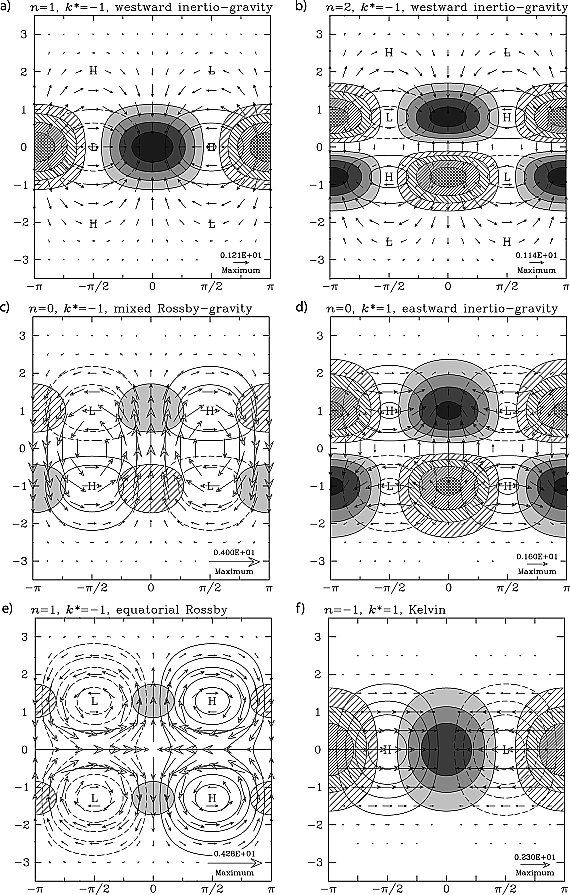
\includegraphics[height=0.7\textheight]{graphics/rog1687-fig-0003.png}\\
Horizontal structures of selected zonally propagating wave solutions to the shallow water equations on an equatorial $\beta$ plane. (Kiladis et al., 2009)
\end{solution}

\section{Python Programming}
Here we demonstrate how to compute a real inner product supplied by a symmetric bilinear form $B$ and carry out Gram-Schmidt Orthogonalization with respect to it. We use Example \ref{exmp:R3innerGS} as the test case. We first define a function to calculate the inner product given two input vectors and the matrix $B$:
\begin{lstlisting}
import numpy as np

def real_inner_prod(u, v, B):
    if np.all(B == B.T): # Check if symmetric
        return(u @ B @ v)
    else:
        print("Not symmetric bilinear form!")
        return(None)   
\end{lstlisting}
Let's check it with that $B$ in Example \ref{exmp:R3innerGS} and $\vec{u} = (1,0,1)^T$, $\vec{v} = (0,2,-1)^T$. Then
\begin{lstlisting}
u = np.array([1., 0., 1.])
v = np.array([0., 2., -1.])
B = np.array([[2., 1., 0.],  
              [1., 2., 1.],
              [0., 1., 2.]])

print(real_inner_prod(u,v,B))    
\end{lstlisting}
gives \verb|2.0| which turns out to be correct. For convenience we also define a function to compute norm, which is simply a wrapped version of \verb|real_inner_prod|:
\begin{lstlisting}
def norm(v, B):
    return(np.sqrt(real_inner_prod(v, v, B)))
\end{lstlisting}
Now come the main part of executing the Gram-Schmidt procedure. The inner loop subtract the parallel components of each previous vector from the current vector and the outer loop iterates the calculation for every vector.
\begin{lstlisting}
def GS_inner_prod(vecs, B):
    """
    Gram-Schmidt Orthogonalization with respect to an inner product (finite-dimensional)
    vecs: A list containing the vectors
    B: The symmetric matrix for the inner product
    """
    n_vecs = len(vecs)
    for jj in np.arange(n_vecs):
        for ii in np.arange(jj):
            vecs[jj] -= real_inner_prod(vecs[jj], vecs[ii], B) / norm(vecs[ii], B)**2 * vecs[ii]
    return(vecs)    
\end{lstlisting}
Trying this with Example \ref{exmp:R3innerGS}
\begin{lstlisting}
vecs = [np.array([1.,0.,0.]), 
        np.array([0.,1.,0.]), 
        np.array([0.,0.,1.])]
print(GS_inner_prod(vecs, B))
\end{lstlisting}
produces
\begin{lstlisting}
[array([1., 0., 0.]), array([-0.5,  1. ,  0. ]), array([ 0.33333333, -0.66666667,  1.        ])]    
\end{lstlisting}
which matches our answer in the example.

\section{Exercises}

\begin{Exercise}
Show that the set of all $n \times n$ (complex) matrices $\mathcal{V} = \mathcal{M}_{n \times n}(\mathbb{C})$ is a vector space and the definition $\langle A, B\rangle = \text{tr}(AB^*)$ satisfies the requirements of an inner product for this vector space. This form of inner product is better known as the \textit{Frobenius inner product}.
\end{Exercise}

\begin{Exercise}
Show that $\vec{u} = (-1,0,2)^T$ and $\vec{v} = (1,-1,1)^T$ in $\mathbb{R}^3$ are orthogonal to each other if an inner product of
\begin{align*}
\langle\vec{u}, \vec{v}\rangle = \vec{u}^TB\vec{v}
\end{align*}
where 
\begin{align*}
B = 
\begin{bmatrix}
2 & 1 & 1 \\
1 & 2 & 1 \\
1 & 1 & 1
\end{bmatrix}
\end{align*}
is used. Also, find the norm $\norm{\vec{u}}$ and $\norm{\vec{v}}$ of both $\vec{u}$ and $\vec{v}$ with respect to this inner product.
\end{Exercise}

\begin{Exercise}
Let $\mathcal{V} = \mathbb{R}^3$. Show that
\begin{align*}
\langle\vec{u}, \vec{v}\rangle = \vec{u}^TB\vec{v}
\end{align*}
where 
\begin{align*}
B = 
\begin{bmatrix}
3 & 1 & -1 \\ 
1 & 3 & 0 \\ 
-1 & 0 & 1
\end{bmatrix}
\end{align*}
is a valid inner product for all $\vec{u}, \vec{v} \in \mathcal{V}$ and turns $\mathcal{V}$ into an inner product space. Hence derive an orthonormal basis for $\mathbb{R}^3$ with respect to this inner product using Gram-Schmidt Orthogonalization. 
\end{Exercise}

\begin{Exercise}
Prove the Triangular Inequality
\begin{align*}
\norm{\vec{u} + \vec{v}} \leq \norm{\vec{u}} + \norm{\vec{v}}
\end{align*}
now for any inner product.
\end{Exercise}

\begin{Exercise}
Show that $x^3$ and $\cos(2x)$ is orthogonal to each other in the $L^2[-\pi, \pi]$ space with respect to the inner product of Equation (\ref{eqn:integralinner}).
\end{Exercise}

\begin{Exercise}
Find the adjoint of $\mathcal{L}[f] = \frac{d}{dx}(x\frac{d}{dx}[f])$ with respect to the inner product of Equation (\ref{eqn:integralinner2})
\begin{align*}
\langle f,g \rangle = \int_a^b w(x) f(x) \overline{g(x)} dx \label{eqn:integralinner2}   
\end{align*}
where $w(x) =$ (a) $1$, and (b) $x$, with $a > 0$.
\end{Exercise}

\begin{Exercise}
Show that given a real inner product induced by $\langle \vec{u},\vec{v} \rangle = \vec{u}^TB\vec{v}$ where
\begin{align*}
B = 
\begin{bmatrix}
1 & 1 \\
1 & 2
\end{bmatrix}
\end{align*}
The linear operator
\begin{align*}
T = 
\begin{bmatrix}
2 & 1 \\
0 & 1
\end{bmatrix}
\end{align*}
is self-adjoint.
\end{Exercise}

\begin{Exercise}
Find the Fourier series of (a) $x^2$, (b) $x^3$ and (c) $4+\sin(3x)+2\cos(8x)$ over $[-\pi, \pi]$.
\end{Exercise}

\begin{Exercise}
Convert the Legendre's Equation
\begin{align*}
(1-x^2) y'' - 2xy' + \lambda y = 0
\end{align*}
into the Sturm-Liouville form, what should be the natural interval such that the corresponding Sturm-Liouville operator is Hermitian? Then, show that when $\lambda = n(n+1)$, $n$ is a non-negative integer, the series solution truncates and produces the Legendre polynomials as its eigenfunctions. Find the first five of them. Alternatively, apply the Gram-Schmidt procedure over the standard polynomial basis over the natural interval to come up with the same set of Legendre polynomials.
\end{Exercise}